%\documentclass[11pt, draft, oneside]{report}
\documentclass[11pt]{report}
\makeindex
\usepackage{ngerman,a4,showidx} %index an seite
%\usepackage{ngerman,a4wide}
%for pdfLaTeX output Bilder als .png speichern:
\usepackage{listings}
\usepackage{nomencl}
\usepackage{framed,color}
\usepackage[pdftex]{graphicx}
% f\"{u}r normales LaTeX->dvi, Bilder als .eps speichern:
\usepackage{graphicx} \DeclareGraphicsExtensions{.eps} %\graphicspath{{bilder/eps/}}

%Definition der Seitengr"osse
\setlength{\textwidth}{15 true cm}
\setlength{\textheight}{22 true cm}
\oddsidemargin  0.5 cm
\evensidemargin 0.5 cm
\topmargin      0 cm

\selectlanguage{german}
%Beispiel fuer ein neues LaTex Kommando
\newcommand{\QSIM}{{\sc QSim}}


\begin{document}

\begin{titlepage}
\begin{center}
  \vspace*{0.5cm}
  {\LARGE Report Studiomesstechnik LU - Group 6} \\
  \vspace{15mm}
  {\huge \bf Laboratory Day 3 - Measurement of DACs and ADCs \\}

  \vspace{15mm}
  {\LARGE Andreas Johann H\"ormer} \\
{\small }Andreas Lebherz\\
Marlene Glawischnig\\
Nepomuk Krenn\\
J\"urgen Schmidt\\ %}
  \vspace{10mm}%15
  -------------------------------------- \\
  \vspace{10mm}%15
  \large
  Institute for signal processing and speech communication \\
  Graz University of Technology \\


  %Vorstand: O.\,Univ.-Prof.\,Dipl.-Ing.\,Dr.\,techn.\,Reinhold Wei{\ss} \\
  \vspace{15mm}%1
  \begin{figure}[!ht]
  \begin{center}
  \centerline{
\includegraphics[width=4cm,keepaspectratio=true]{TULogoneu}}
  \end{center}
  \end{figure}
  \vspace{10mm}
Supervisor: DI Wolfgang Truppe \\
  %Begutachter: O.\,A.o.Univ.-Prof.\,Dipl.-Ing.\,Dr.\,techn.\,Eugen Brenner \\
  %\vspace{5mm}
  %Betreuer: Univ.-Ass. Dipl.-Ing.\,Dr.\,techn.\,N. N.\\
  \vfill
  %\newline
  %\normalsize
  audio studio of TU Graz, 11.03.2015
  \vspace{0.5cm}
\end{center}
\end{titlepage}

% Die Titelseite ist immer in Deutsch (austrian), danach h\"{a}ngt es von der
% Sprache der Diplomarbeit ab. Jedenfalls muss eine Kurzfassung und
% ein Abstract existieren

%\thispagestyle{empty} 
%\selectlanguage{english}


\newpage
\selectlanguage{english}
\vspace*{2.2 cm}
{\Large
\noindent
{\bf Abstract}} \\
\vspace*{0.3 cm}

\noindent
Main target of this laboratory was the measurement of different DACs and ADCs of the fully digital mixing panel LAWO $mc^2 66$. Additionally preamplifiers of a high quality input compared to standard inputs were measured. Measurements were done qualitatively in terms of dynamic ranges and frequency characteristics.\\
This report consists of 28 pages. 


%\newpage


%\selectlanguage{english}
%\vspace*{2.2 cm}
%{\Large
%\noindent
%{\bf STATUTORY DECLARATION}} \\
%\vspace*{0.3 cm}

%\noindent
%I declare that I have authored this thesis independently, that I have not used other than the declared sources / %resources, and that I have explicitly marked all material which has been quoted either literally or by content from %the used sources.
%\vspace*{0.3 cm}

%\vspace{2 cm}

%\noindent ..............................\hfill ...........................................


%\noindent date  \hfill (signature)
\renewcommand{\nomname}{List of abbreviations}
\setlength{\nomlabelwidth}{.50\hsize}
\renewcommand{\nomlabel}[1]{#1 \dotfill}
\setlength{\nomitemsep}{-\parsep}
\makenomenclature

\newpage
\selectlanguage{english}
%\newpage
%\vspace*{2.2 cm}
%{\Large
%\noindent
%{\bf Danksagung}} \\
%\vspace*{0.3 cm}
% OPTIONAL

%\noindent
%Diese Diplomarbeit wurde im (Studien)Jahr am Institut f\"{u}r
%Technische Informatik an der Technischen Universit\"{a}t Graz
%durchgef\"{u}hrt.

%\smallskip
%Danksagung an alle am Institut bzw. bei Firmen, die geholfen
%haben....

%\medskip
%Danksagung an Freunde und Freundinnen f\"{u}r das Verst\"{a}ndnis, ebenso
%den Eltern und allen sonstigen Sponsoren....

%\vspace{2 cm}

%
%\noindent Graz, im Monat Jahr \hfill Name des Diplomanden

\newpage
% Inhaltsverzeichnis
\tableofcontents  

% Tabellenverzeichnis
% OPTIONAL
%




\listoffigures 

% Abbildungsverzeichnis
% OPTIONAL
%\listoftables

%Seitennummerierung am Kopf inkl. Kapitel"uberschrift
\pagestyle{headings}

%---------------------------------------------------------------------------------------------------------
%---------------------------------------------------------------------------------------------------------
\chapter{Preamble}
% Einleitung ist Kapitel 1
\label{kap:Einleitung} 

%---------------------------------------------------------------------------------------------------------
\section{Motivation}
Due to high computation speeds and huge possibilities for postprocessing techniques almost everything became digital. For digital audio a conversion between the digital and the analog domain and vice versa is inevitable. As ADCs and DACs are the links between those two domains they affect the resulting sound quality very much. For best results a high quality of conversion components is needed. 

%---------------------------------------------------------------------------------------------------------
\section{Purpose}
The main purpose of the laboratory was the measurement of important parameters of conversion components. Parameters like dynamic range and frequency responses at different preamplifier gains as well as linearity of converters is shown. A FFT analysis of noise was made.


%---------------------------------------------------------------------------------------------------------
%---------------------------------------------------------------------------------------------------------
\chapter{DAC measurements}
\section{Introduction}
\subsection{DAC}
A digital-analog-converter (DAC) converts a digital signal (discrete in time and amplitude) into an analog signal. In order to produce sound this analog signal can be used to drive an amplifier and be connected to loudspeakers. Typical DACs for audio applications are low speed components with high resolution. As every conversion between digital and analog domains can degrade signals and add possible distortions, some parameters are useful to determine the quality of converters:
\begin{itemize}
\item resolution\\
The resolution (in bit) is the number of possible output states in the amplitude domain. The higher the resolution is, the more different output states can be created. The difference between different states become lower and the analog signal becomes finer. In audio applications the resolution is also known as audio bit depth.
\item maximum sampling rate\\
The sampling rate defines the number of changes of the output signals can be made per second.
\item monotonicity\\
This describes the linearity of the converter. When the digital input increases, the analog output should have the ability to move the same amount upwards without doing anything else (dips, ripples, ...).
\item THD+N\\
The total harmonic distortion and noise is a measurement of the unwanted harmonics produced by the converter. Especially for small signals created by the converter could affect the output signal significantly. 
\item dynamic range\\
This parameter describes the difference between the lowest output level and the highest output level which can be driven by the analog output. The lowest level is often given by the noise floor.

\end{itemize}
\section{Measurements}
	\subsection{Experimental setup}
		\subsubsection{Equipment}
\begin{itemize}
\item AudioPrecision sys.2722
\item AudioPrecision Software v3.3 (build118)
\item PC (Windows 7 32bit)
\item SSL amplifier
\item DALLIS DAC slots
\begin{itemize}
\item 942/84: line out channel 24 (AR)
\item 941/83: line out channel 24 (RP1)
\item 942/02: HQ monitor channel 6 (RP1)
\item 942/61: phones 4 (RP1)
\end{itemize}
\end{itemize}
The experimental setup for this measurement can be seen in figure \ref{fig:dacstructure}. A digital signal is sent out with AudioPrecision and routed to the DALLIS. For that reason the AP AES2 was connected to AES3 input 1 right at the patchbay. There different output channels were tested. The analog signal is routed back to the analog input of the AudioPrecision system. 
\begin{figure}[htbp]
\begin{center}
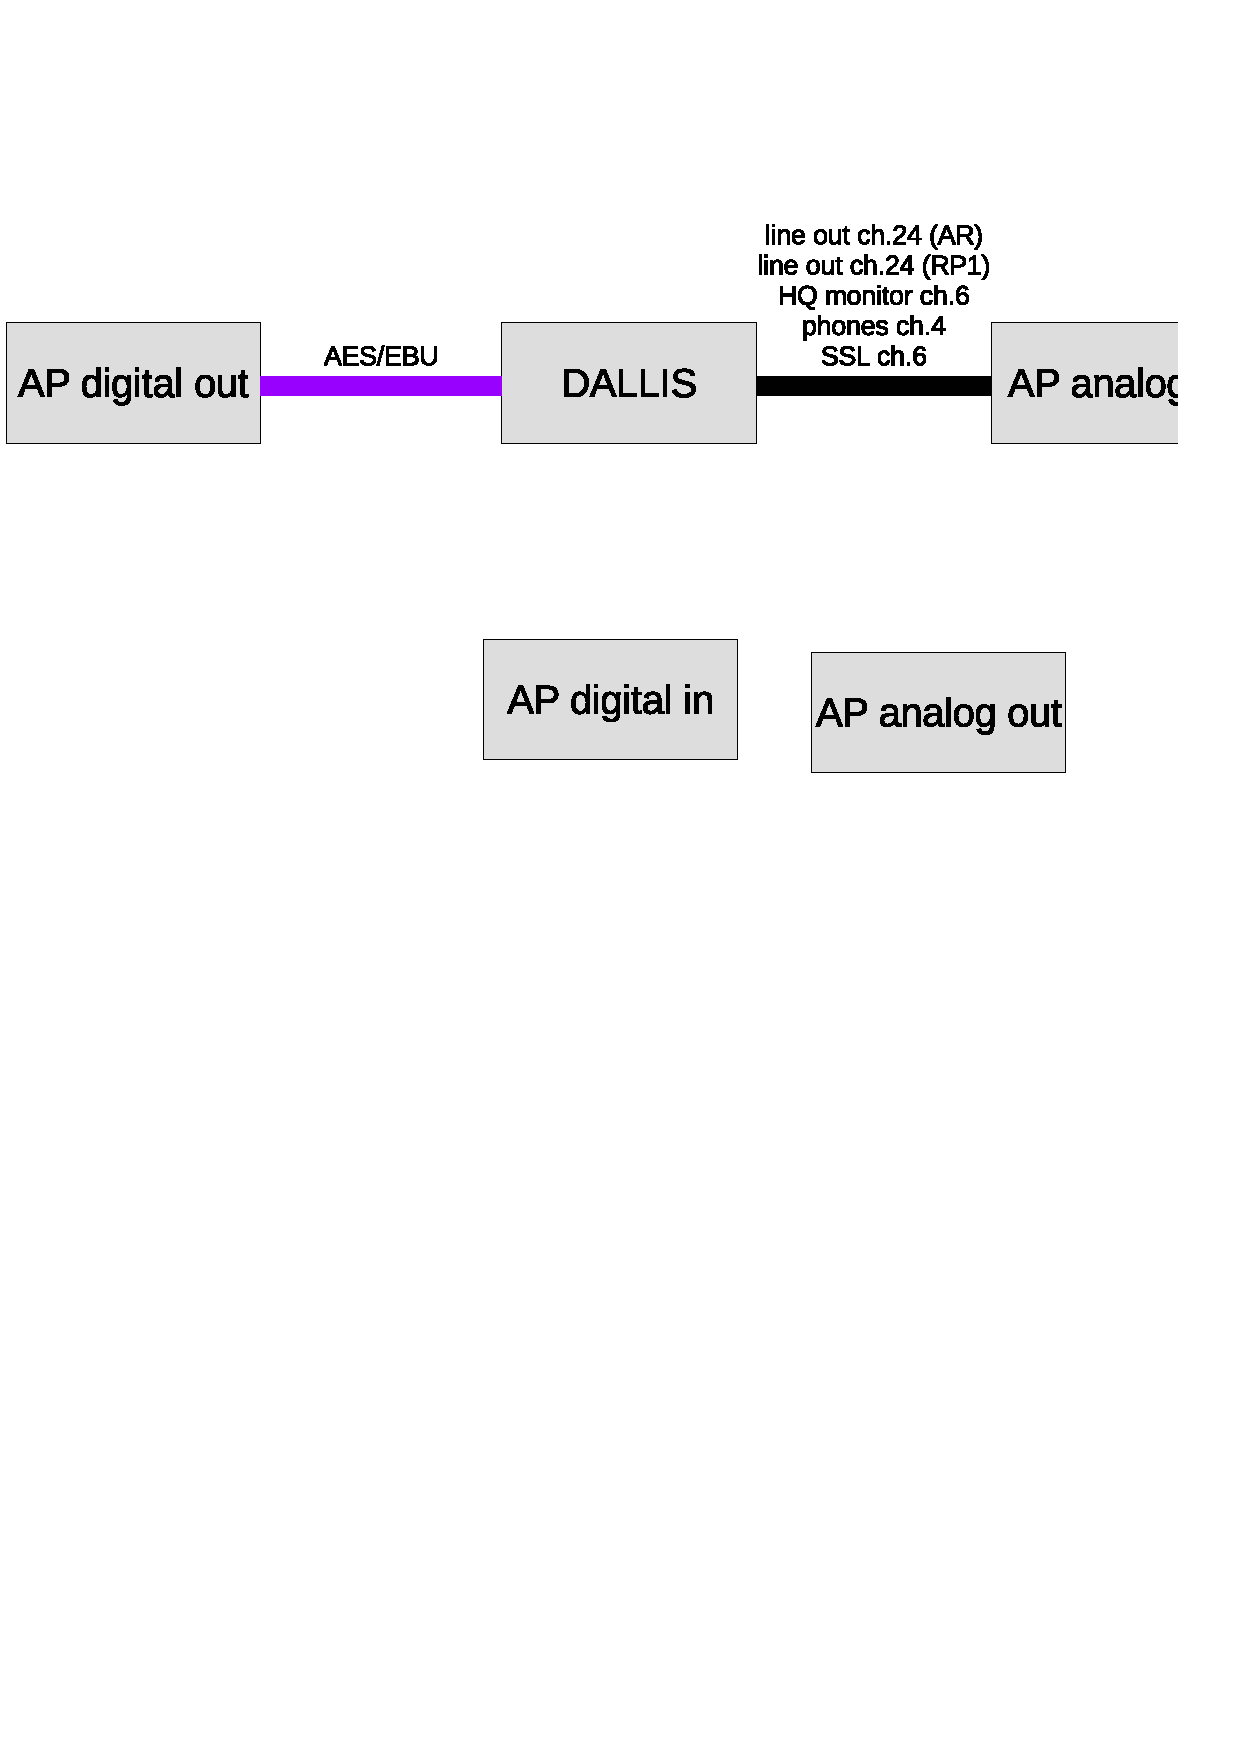
\includegraphics[width=14cm,keepaspectratio=true]{DACstructure}
\caption{experimental setup for DAC measurement}
\label{fig:dacstructure}
\end{center}
\end{figure}
\subsubsection{measurement of frequency response}
The frequency response was measured as in the analog domain. The frequency sweep was done with following configuration:\\
AP digital generator $\rightarrow$ frequency $\rightarrow$ frequency sweep.\\
measured frequency range: $10Hz < f < 30kHz$\\
The digital output was set to a resolution of 24 bits at an output voltage of 5V. All other values were set to default values. As every output channel had different levels, the output levels of AP were adapted. The values can be found in tabular \ref{tab:dacvalues}.
\begin{table}
\begin{center}
\begin{tabular}{|c||c|c|}
\hline 
output channel  & 	output level [$dB_{FS}$]&		input level [$dB_u$]\\ \hline
line out ch.24 (AR) &	-18 &	+6\\
line out ch.24 (RP1) &	-18 &		+6\\
HQ monitor ch.6 &	-9 		& +6\\
phones ch.4 &	-15 &	+6\\
\hline
\end{tabular}
\caption{values for output and input levels for DAC measurements}
\label{tab:dacvalues}
\end{center}
\end{table}
\begin{leftbar}
\textit{ Note:\\
A measurement of phase shifts is not possible when driving the system with a digital output signal.}
\end{leftbar}
\begin{leftbar}
\textit{ Note:\\
When measuring the frequency response it has to be checked that every device uses the same sampling frequency. Otherwise resampling will occur and the frequency response will have slopes in unexpected frequency ranges.}
\end{leftbar}
\begin{leftbar}
\textit{Note:\\
It seemed that it is not possible to measure line out channel 24 (RP1), because it seemed to be connected directly to the talkback channel. After some search it turned out, that channel 24 was not mounted beside channel 23, but on patchbay 2.}
\end{leftbar}
\subsubsection{measurement of dynamic range}
The dynamic range was measured using a 1kHz sine wave and sweeping the amplitude, starting at $-130dB_{FS}$, as end amplitude $0dB_{FS}$ was chosen. As analyzer LevelA was chosen.
\subsubsection{FFT analysis}
The FFT analysis (digital analyzer $\rightarrow$ FFT) was done with a window length of 32768 and a sampling frequency of 262kHz. The results of 16 FFTs were averaged for better graph generation. The FFT was done using a 10kHz sine wave and shaped dithering for noise shaping.

	\subsection{Results}
In figure \ref{fig:da10} the frequency responses of the DACs can be seen, details are shown in figure \ref{fig:dafreqvergleich}. Figure \ref{fig:dadynvergleich} shows the different dynamic ranges of the DACs, the FFT analysis can be found in figure \ref{fig:fft}. High resolution full scale images forprinting purposes are listed in appendix A.

\begin{figure}[htbp]
\begin{center}
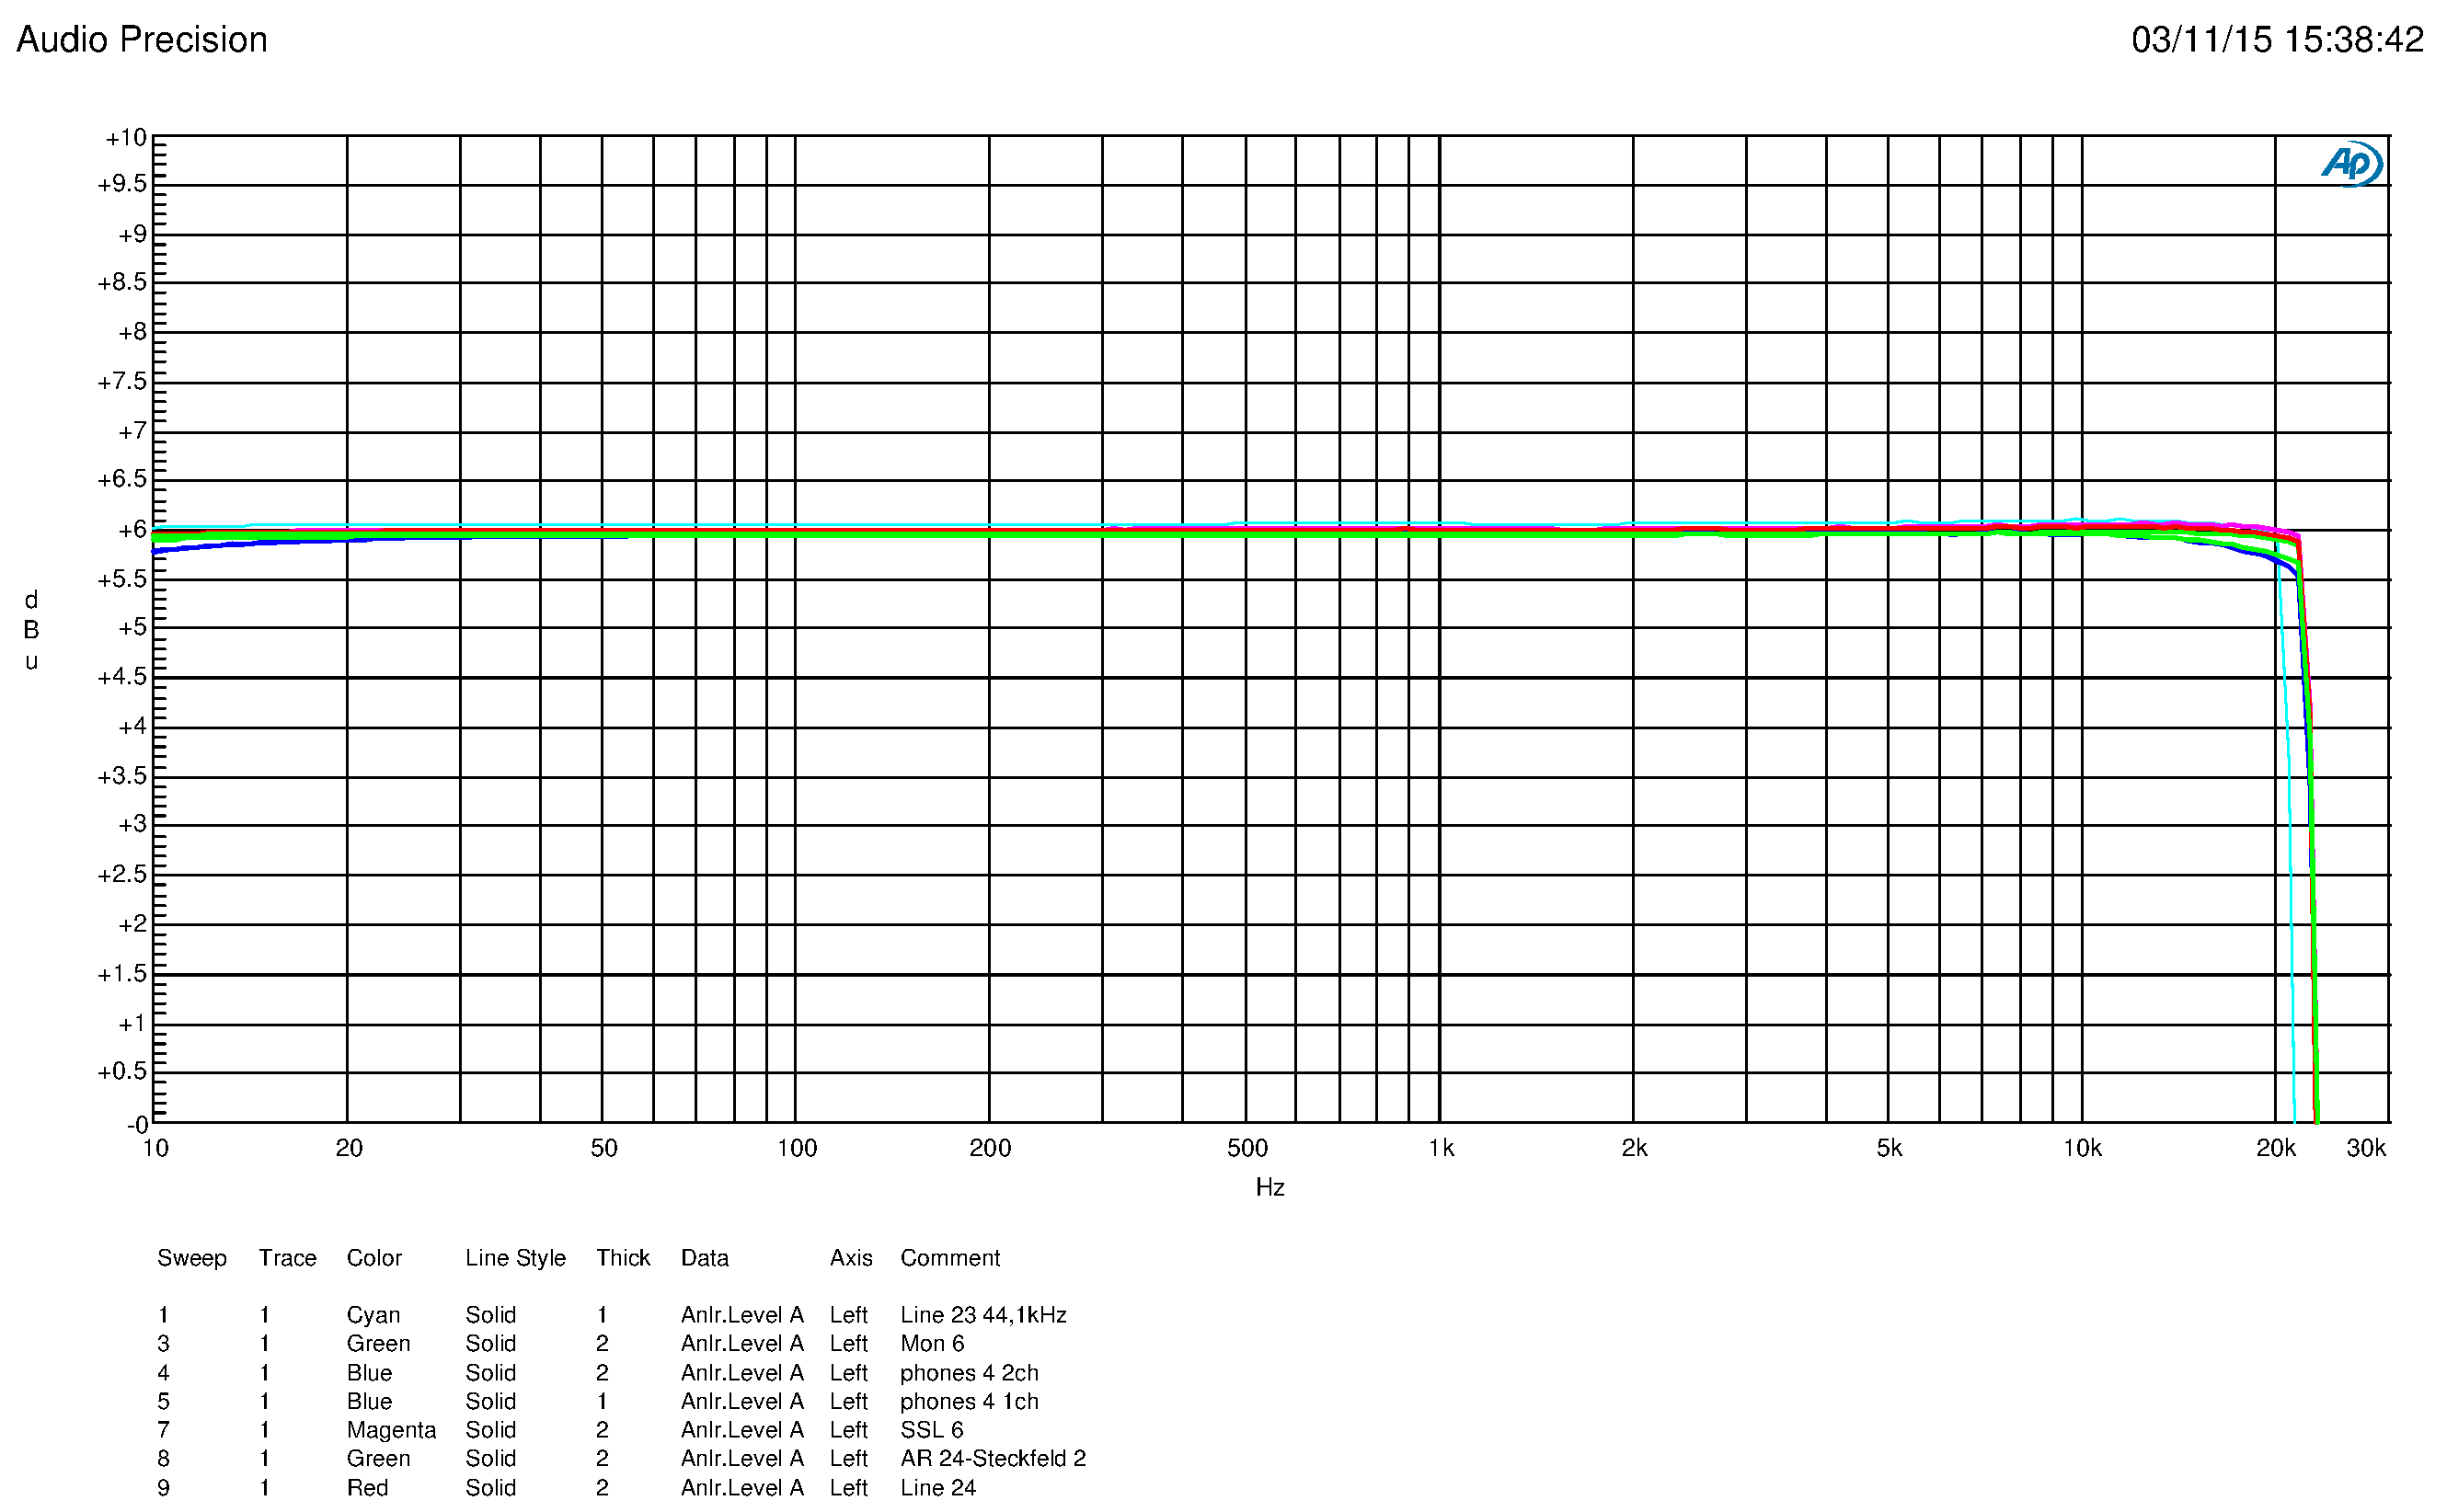
\includegraphics[width=14cm,keepaspectratio=true]{DAWandlerVergleich10dB}
\caption{frequency responses of different DACs}
\label{fig:da10}
\end{center}
\end{figure}

\begin{figure}[htbp]
\begin{center}
\includegraphics[width=14cm,keepaspectratio=true]{DaWandlerVergleich}
\caption{detailed frequency responses of different DACs}
\label{fig:dafreqvergleich}
\end{center}
\end{figure}

\begin{figure}[htbp]
\begin{center}
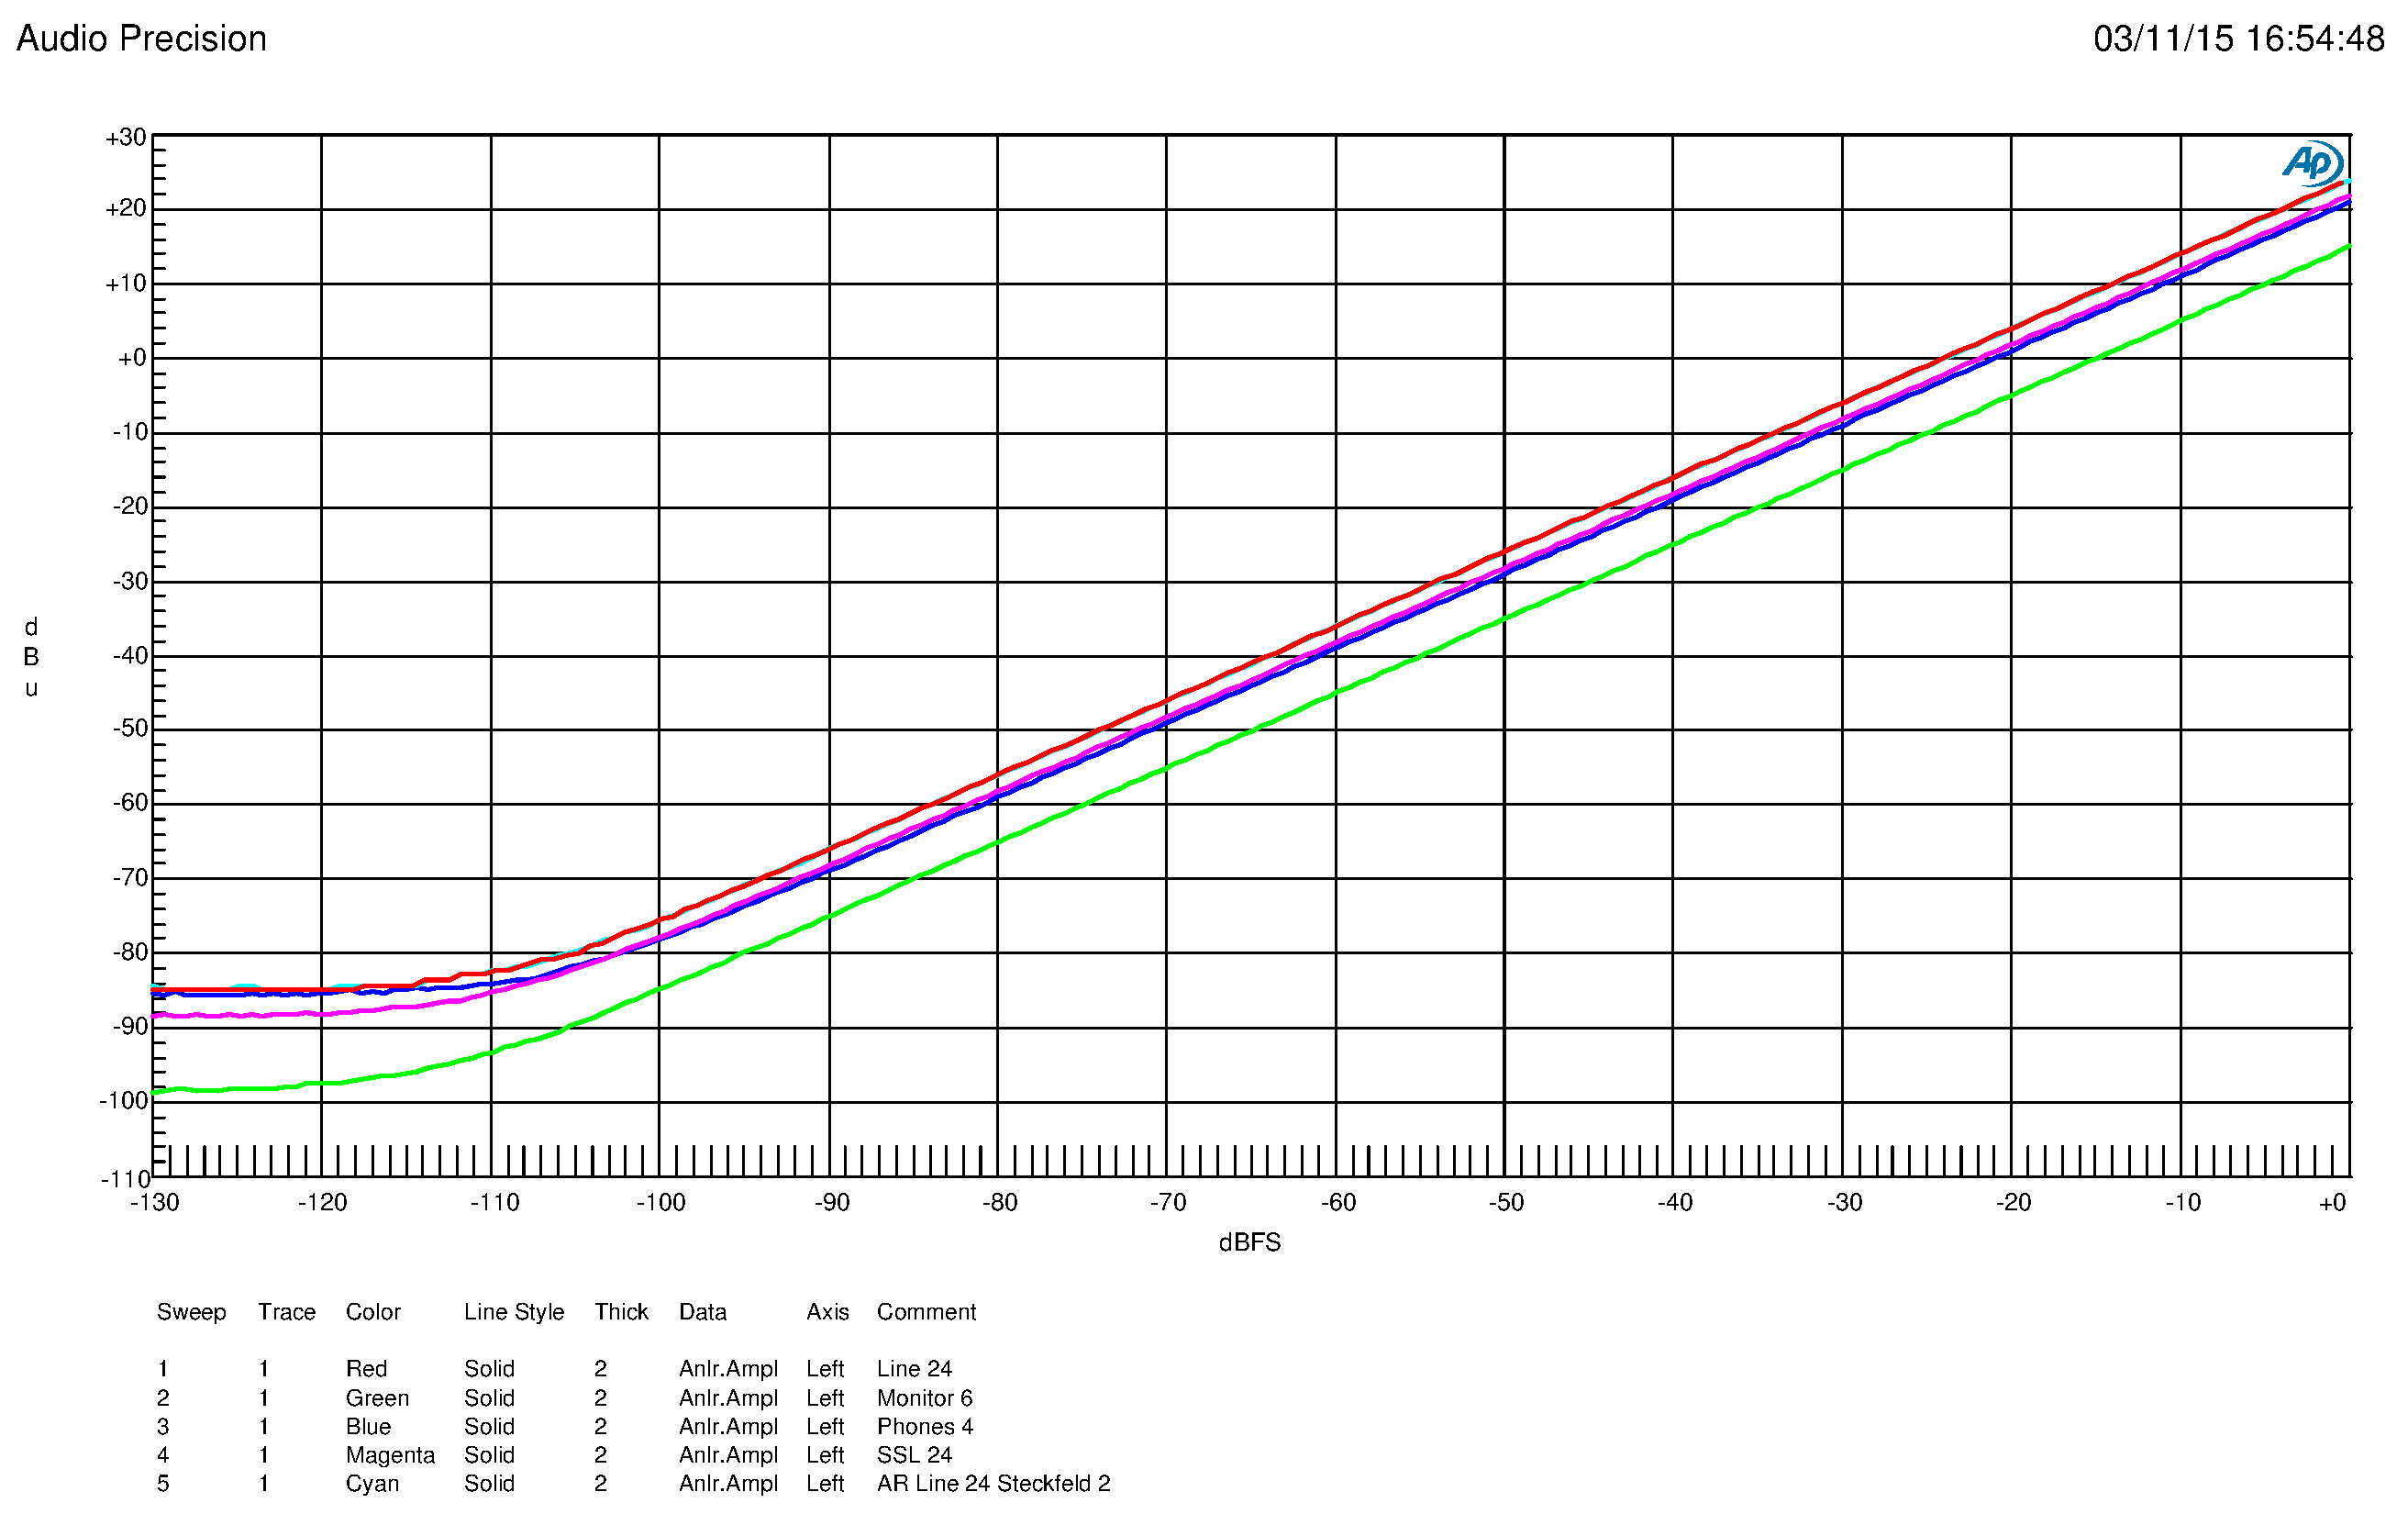
\includegraphics[width=14cm,keepaspectratio=true]{Dynamikvergleich}
\caption{dynamic ranges of different DACs}
\label{fig:dadynvergleich}
\end{center}
\end{figure}

\begin{figure}[htbp]
\begin{center}
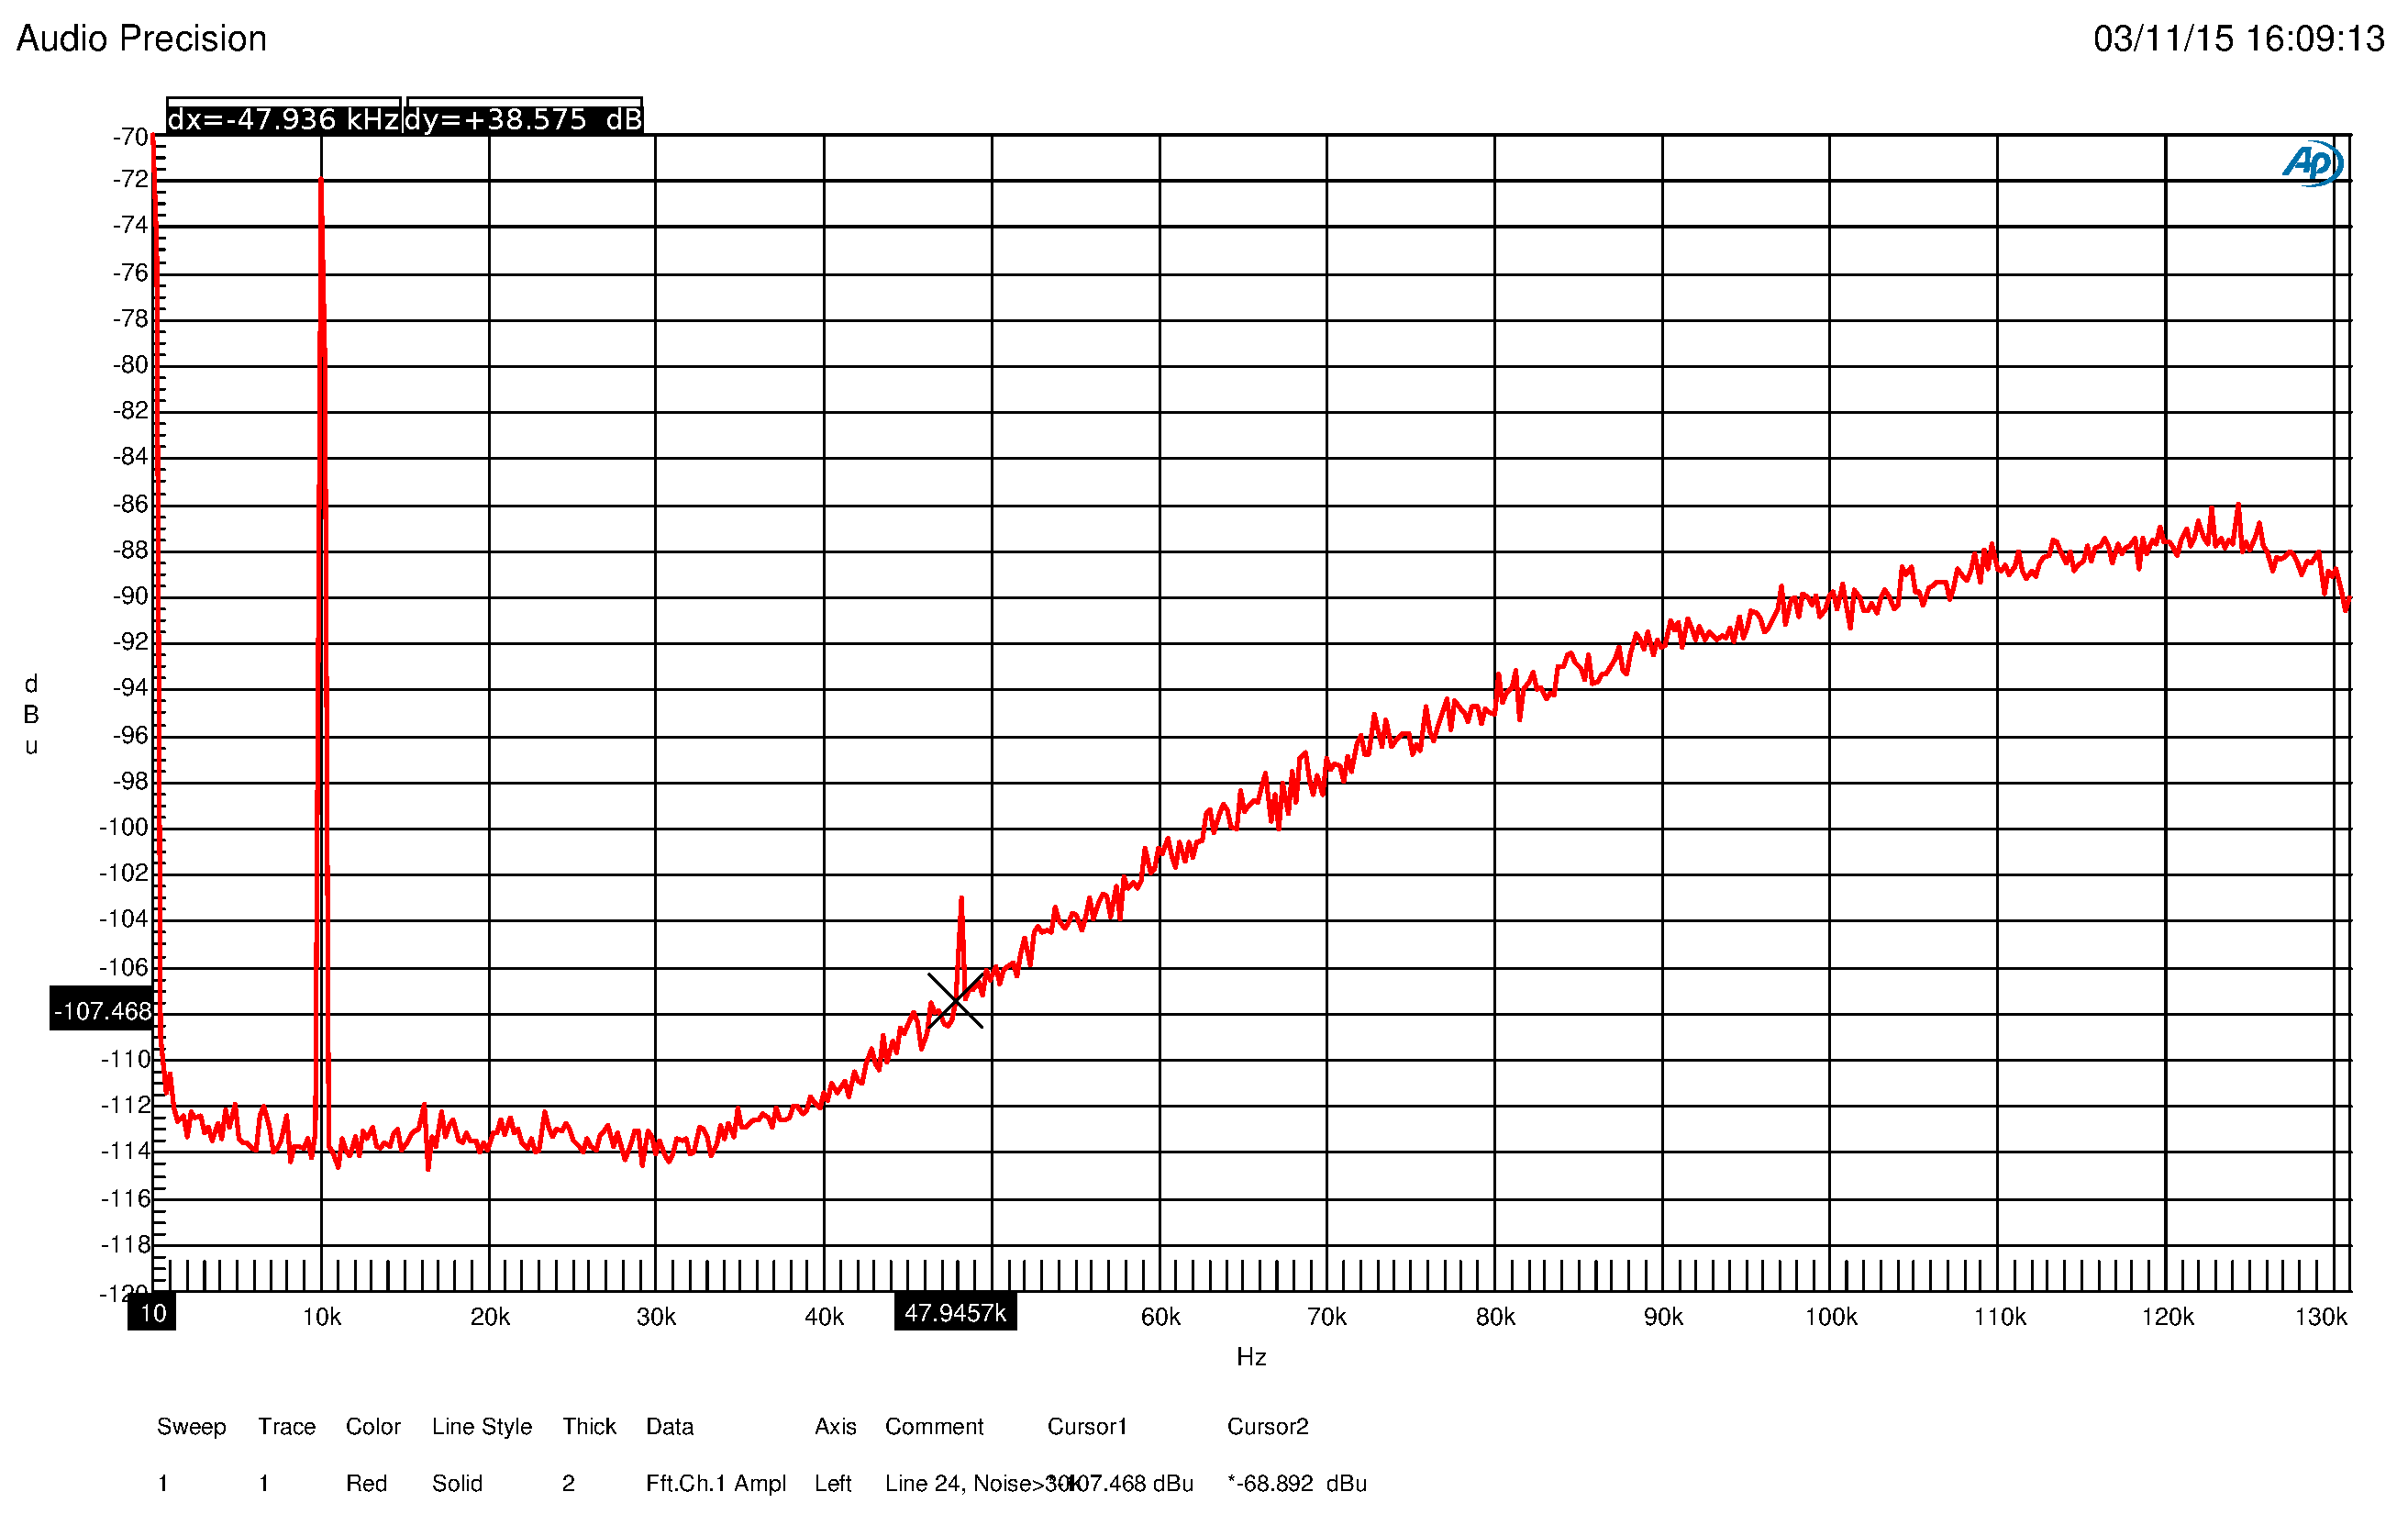
\includegraphics[width=14cm,keepaspectratio=true]{FFTrauschen}
\caption{FFT of line24 signal}
\label{fig:fft}
\end{center}
\end{figure}

	\subsection{Discussion}
In figure \ref{fig:da10} the frequency response of the different DACs are shown. It can be obtained that the amplitude distributions are almost flat over the whole frequency range. At about 21kHz a steep slope down can be seen, which occurs because this range contains half of the sampling frequency (44.1kHz). A lower -3dB cut-off frequency couldn't be measured because it's lower than 10Hz and so lower than the working range of AudioPrecision. When zooming in at the upper part (figure \ref{fig:dafreqvergleich}) some ripples can be seen. They are expected and usual for filters with steep slopes. It can also be obtained that the frequency response is not completely flat when zooming in, but in a negligible amount (left dB scale).\\
The dynamic ranges seen in figure \ref{fig:dadynvergleich} are over a wide range. It can be obtained that the amplification is up to the $0dB_{FS}$-limit, the lower limit is given by the noise floor. It can also be seen that the amplification is completely linear. The measured dynamic ranges are listed in tabular \ref{tab:dadynrange}. An interesting aspect is that the dynamic of the monitor out is slightly lower than the others, but doesn't need to have so much output power.\\
When looking at the FFT analyis in figure \ref{fig:fft} the 10kHz sine wave can be determined easily. It also can be seen that the noise is shaped, and energy from the low, more hearable frequency ranges, is moved to higher frequencies, which don't affect the human hearing as much as at low frequencies.
\begin{table}
\begin{center}
\begin{tabular}{|c|c|}
\hline 
output channel  & 	dynamic range	\\	 \hline
line out ch.24 (AR) &	105dB \\
line out ch.24 (RP1) &	105dB \\
HQ monitor ch.6 &	108dB	\\
phones ch.4 &	102dB \\
SSL & 106dB \\
\hline
\end{tabular}
\caption{values for output and input levels for DAC measurements}
\label{tab:dadynrange}
\end{center}
\end{table}


%---------------------------------------------------------------------------------------------------------
%---------------------------------------------------------------------------------------------------------
\chapter{ADC/preamplifier measurements}
\section{Introduction}
\subsection{ADC}
An analog-digital-converter converts an analog signal to a digital signal by sampling at discrete times and quantization of the analog signal to discrete amplitudes. Some important parameters for ADC quality measurements are
\begin{itemize}
\item resolution\\
The resolution of an ADC measures the number of quantization steps. Each analog value is set to the nearest quantization step. The higher the resolution is, the higher is the accuracy of the signal in the digital domain.
\item sampling rate\\
This parameter describes the number of time steps per second for quantization. For higher rates the signal can be converted more often and represented with more accuracy.
\item sampling time\\
The sampling time is a parameter which defines the time between sampling at the analog input and providing the digital value at the digital output.
\item jitter\\
The jitter regarding to ADCs measures the time difference between the optimal sampling point and the actual sampling point. For high quality ADCs this parameter should be very low.
\end{itemize}
\subsubsection{Quantization}
Quantization is the process of mapping a continuous signal to a countable set of values. The simplest way to quantize a signal is to round the sampled value to the nearest digital amplitude. Figure \ref{fig:quantization}  shows the quantization process. At discrete time steps the value of the input signal is measured and rounded to the nearest discrete value (green and yellow curve). The difference between those two signals is called quantization error or quantization noise and is shown in the red curve. As it can be seen quantization is a lossy process. The maximum error of quantization is always half of the step size between two symbols. The dynamic of quantization increases with every bit with
\begin{equation}
dyn_{[dB]}=20\cdot log(2^Q) \approx 1.761 + 6.02\cdot Q [dB]
\end{equation}
$$Q....number\; of\; bits$$
\begin{figure}[htbp]
\begin{center}
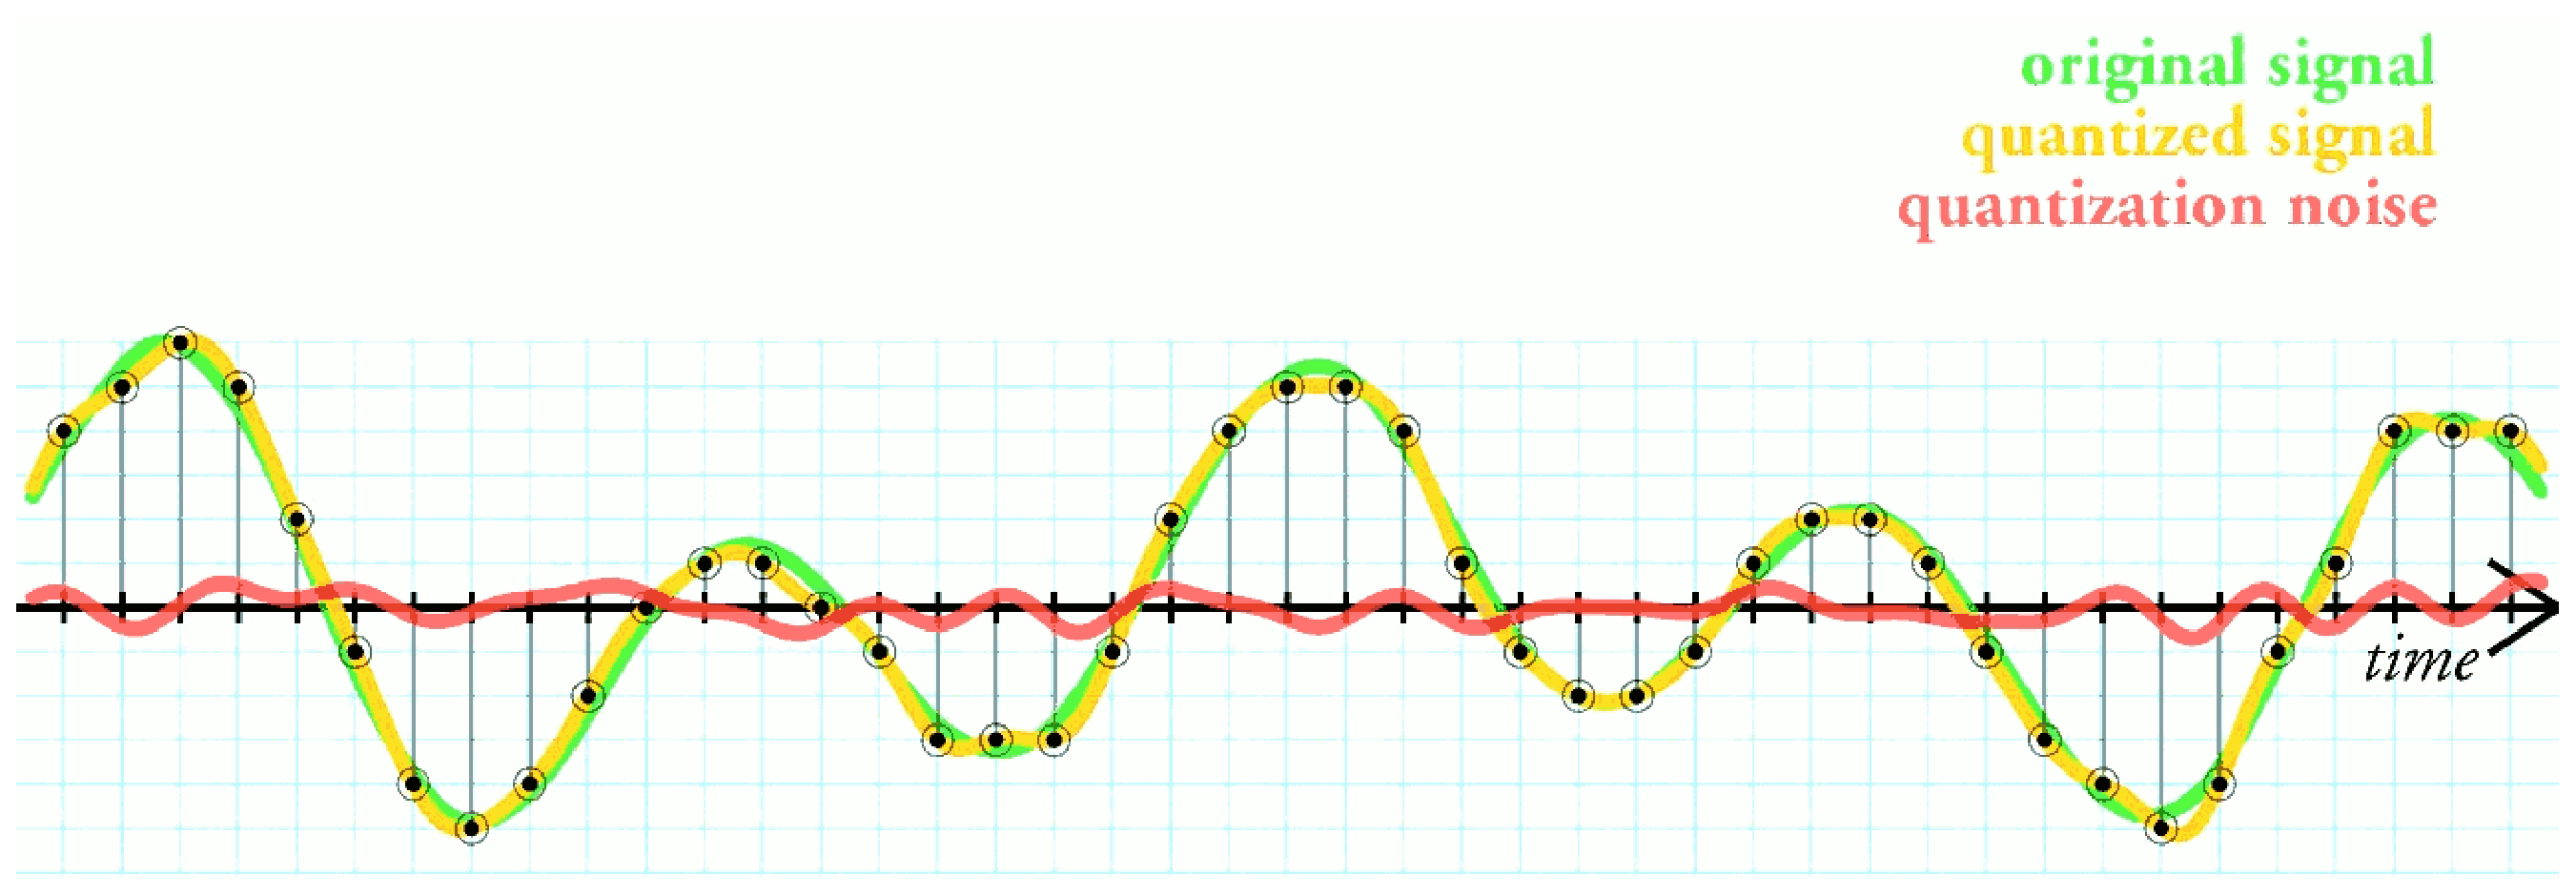
\includegraphics[width=14cm,keepaspectratio=true]{quantization}
\caption{analog-digital conversion of an analog signal}
\label{fig:quantization}
\end{center}
http://upload.wikimedia.org/wikipedia/commons/thumb/b/b8/Quantization\_error.png/500px-Quantization\_error.png
\end{figure}
At low amplitudes it can occur that the analog signal can not be quantized properly due to low resolution. In such case, additional dither can be used.
\subsubsection{Dithering}
Dithering describes the process of adding additional noise to a signal. In terms of audio engineering it helps to break up correlated error signals from quantization steps. Random noise is typially less objectionable than harmonic tones, produced by quantization. Dithering helps to break up those periodic cycles. Addionally noise shaping can be used. Noise energy at low frequency can be shaped and moved to higher frequency ranges, where the human listening is less affected.
\section{Measurements}
	\subsection{Experimental setup}
The experimental setup for measuring a standard quality microphone input as well as a HQ microphone input of DALLIS is shown in figure \ref{fig:adcstructure}. The analog output of AP was set to $-64dB_u$, the digital input had to have a level of $-18dB_{FS}$. The frequency responses were measured using preamplifier gains 70dB, 55dB, 40dB, 25dB and 16/20dB (HQ, standard quality). The frequency sweep for measuring the frequency response had 200 steps from 10Hz to 30kHz. The amplitude sweep for measuring the dynamic range started at $-140dB_{FS}$ and ended at $30-gain\; dB_{FS}$. The sweeps were done using the analog generator of AP.
\begin{figure}[htbp]
\begin{center}
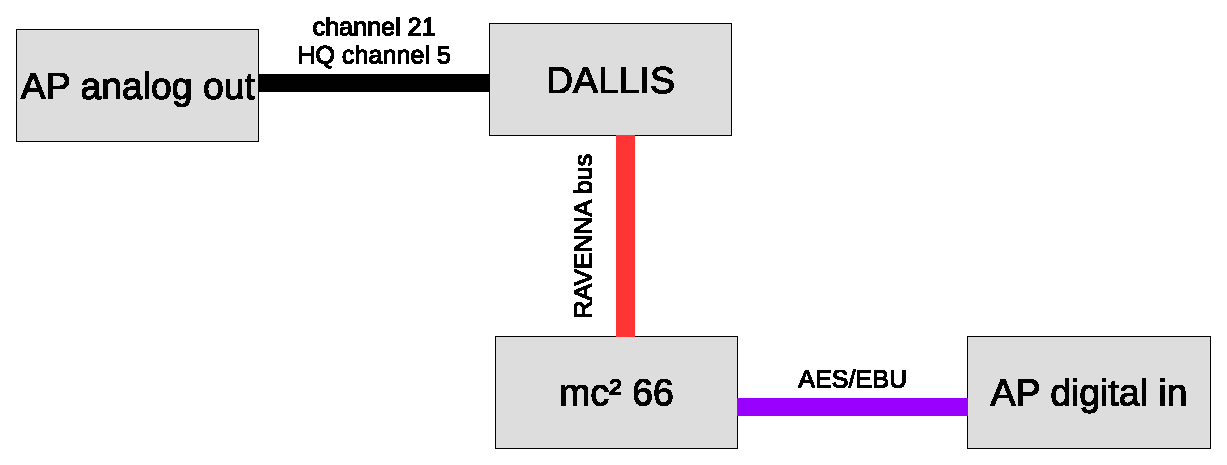
\includegraphics[width=14cm,keepaspectratio=true]{ADCstructure}
\caption{experimental setup for ADC measurement}
\label{fig:adcstructure}
\end{center}
\end{figure}
		\subsubsection{Equipment}
\begin{itemize}
\item AudioPrecision sys.2722
\item AudioPrecision Software v3.3 (build118)
\item PC (Windows 7 32bit)
\item $LAWO \; mc^2 66$
\item DALLIS DAC slots
\begin{itemize}
\item 941/53: HQ channel 5 (AR)
\item 942/84: channel 21 (AR)
\end{itemize}
\end{itemize}
	\subsection{Results}
Figure \ref{fig:adlawo} shows the frequency response of the microphone channel as well as the high quality microphone channel with different preamplifier gains, a more detailed view is given in figure \ref{fig:adlawovergleich}. The THD+N of the standard quality input is shown in figure \ref{fig:adthd}, the THD+N of the high quality microphone input in figure \ref{fig:adhqthd}.
\begin{figure}[htbp]
\begin{center}
\includegraphics[width=14cm,keepaspectratio=true]{LAWOVorverstaerker5u21dB}
\caption{LAWO ADC and preamplifier}
\label{fig:adlawo}
\end{center}
\end{figure}

\begin{figure}[htbp]
\begin{center}
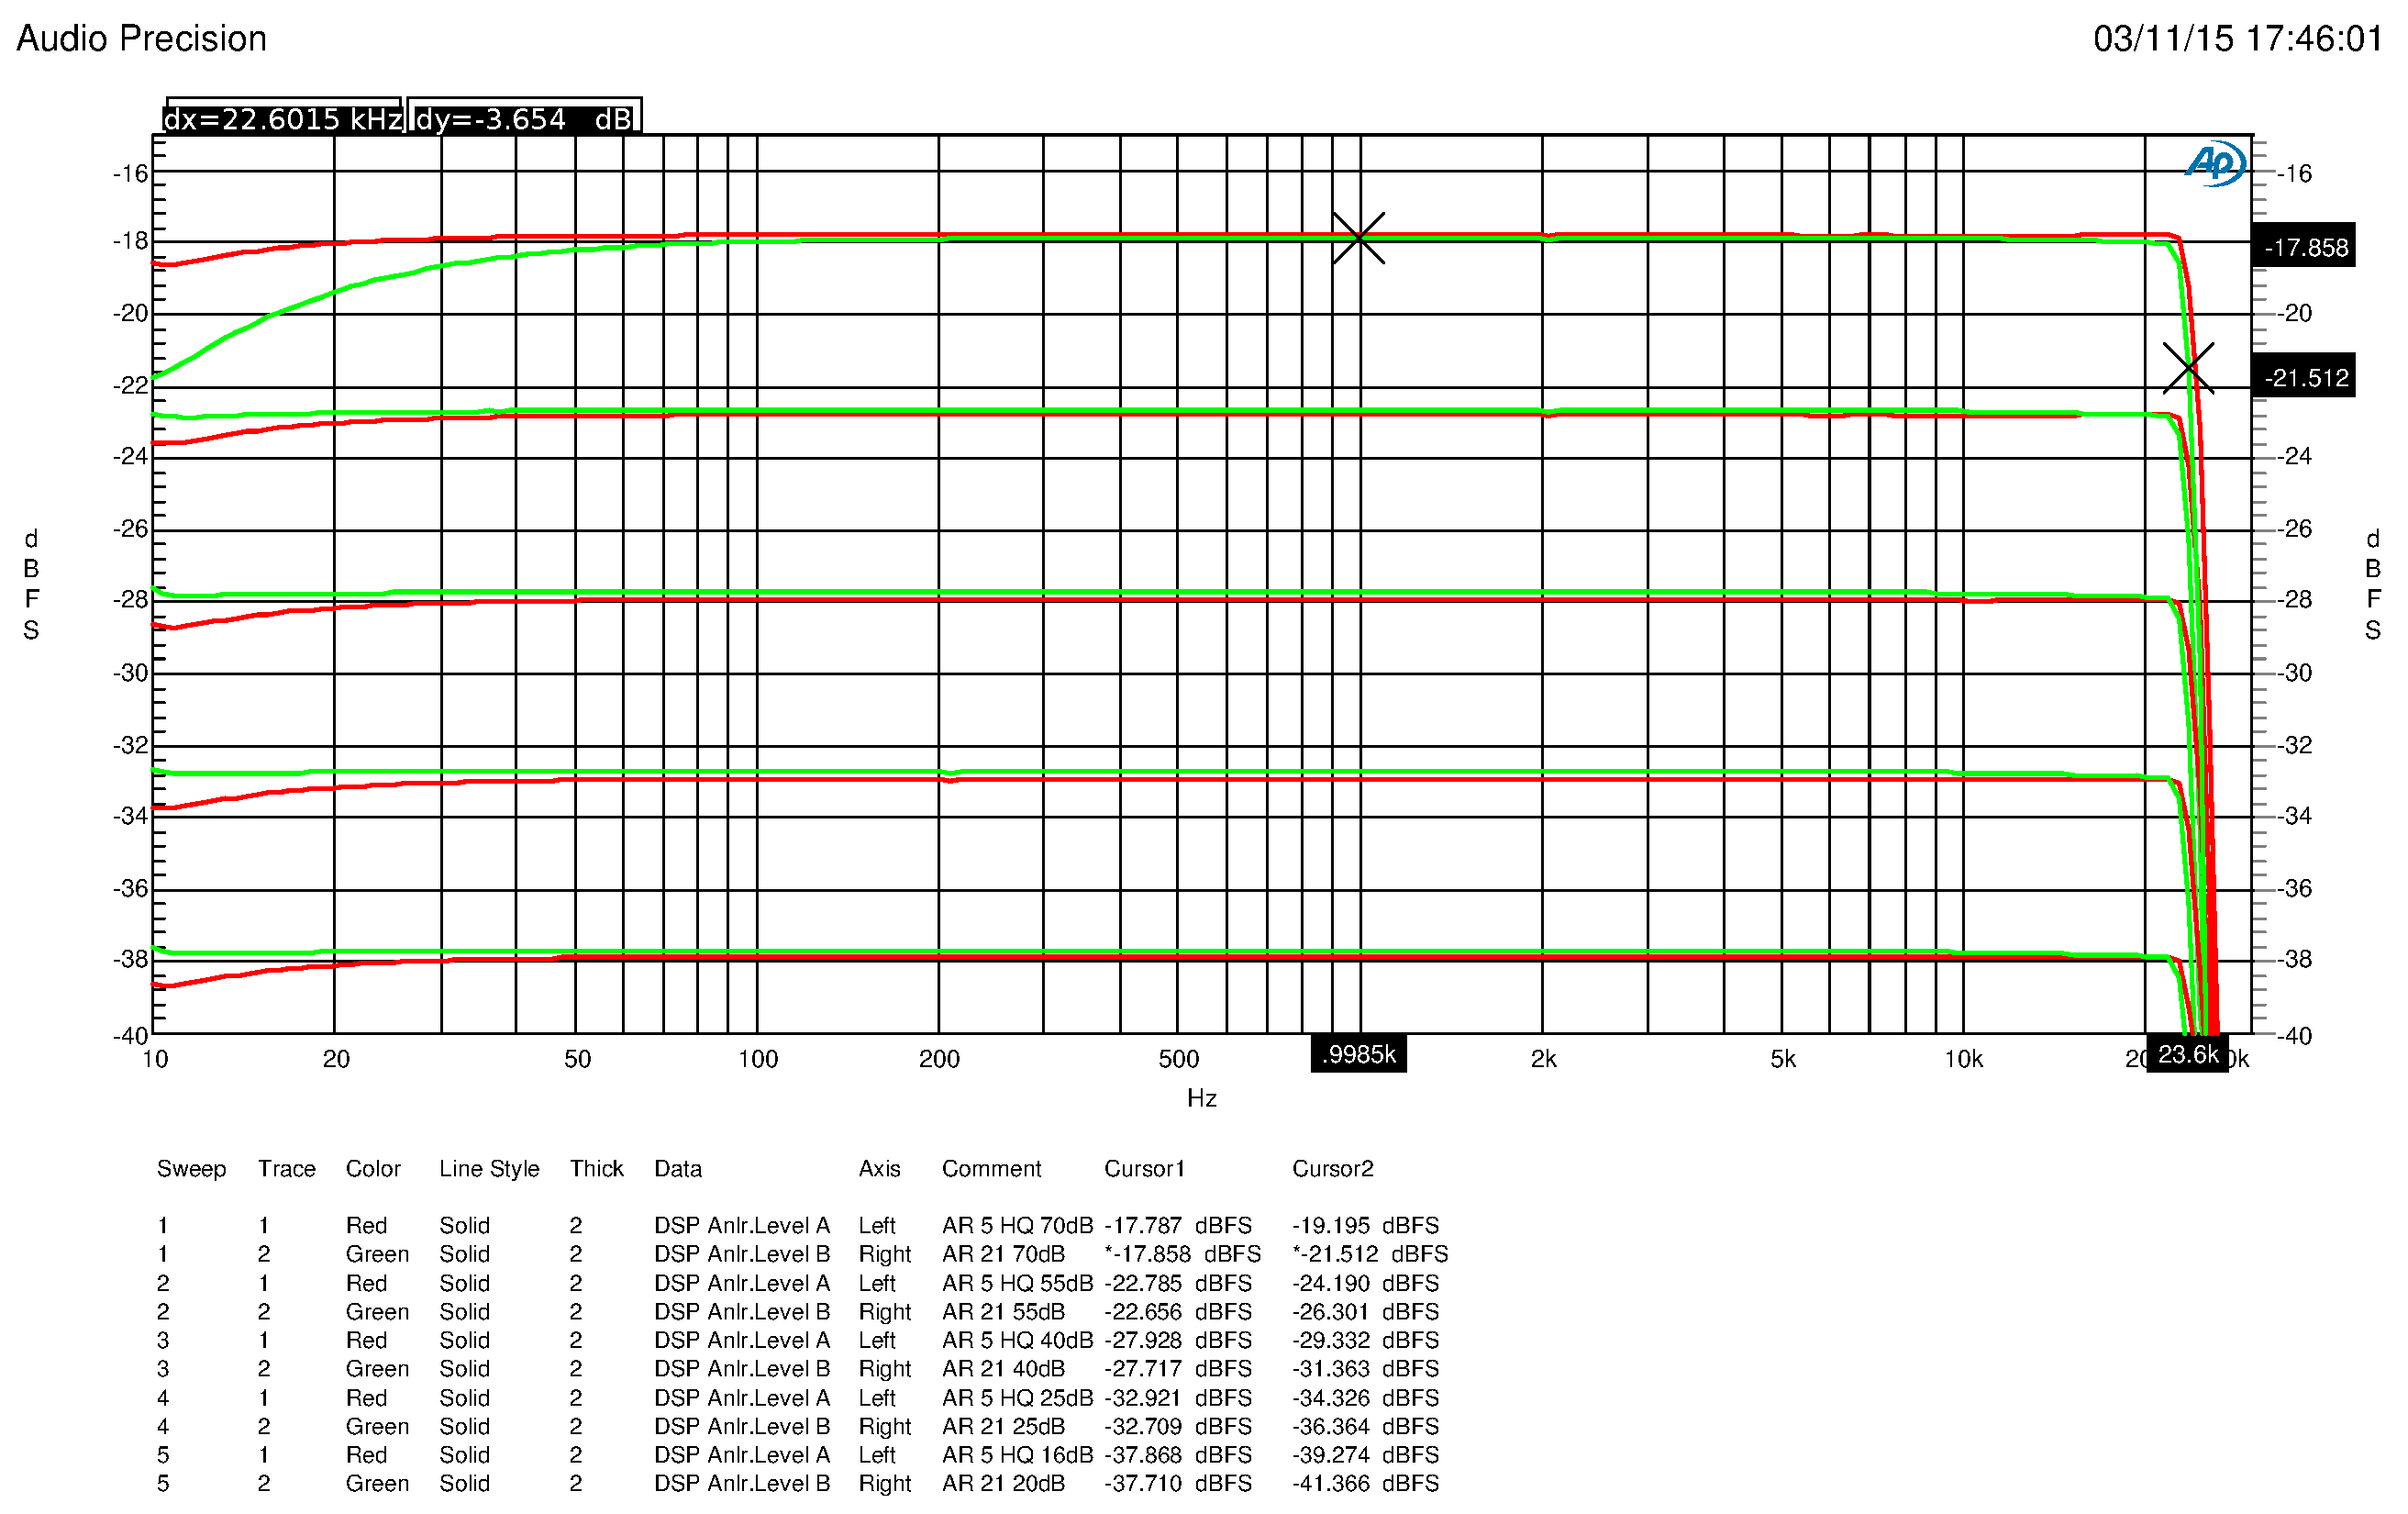
\includegraphics[width=14cm,keepaspectratio=true]{LAWOVorverstaerker5u21dBVergleichszoom}
\caption{LAWO ADC and preamplifier detailed view}
\label{fig:adlawovergleich}
\end{center}
\end{figure}

\begin{figure}[htbp]
\begin{center}
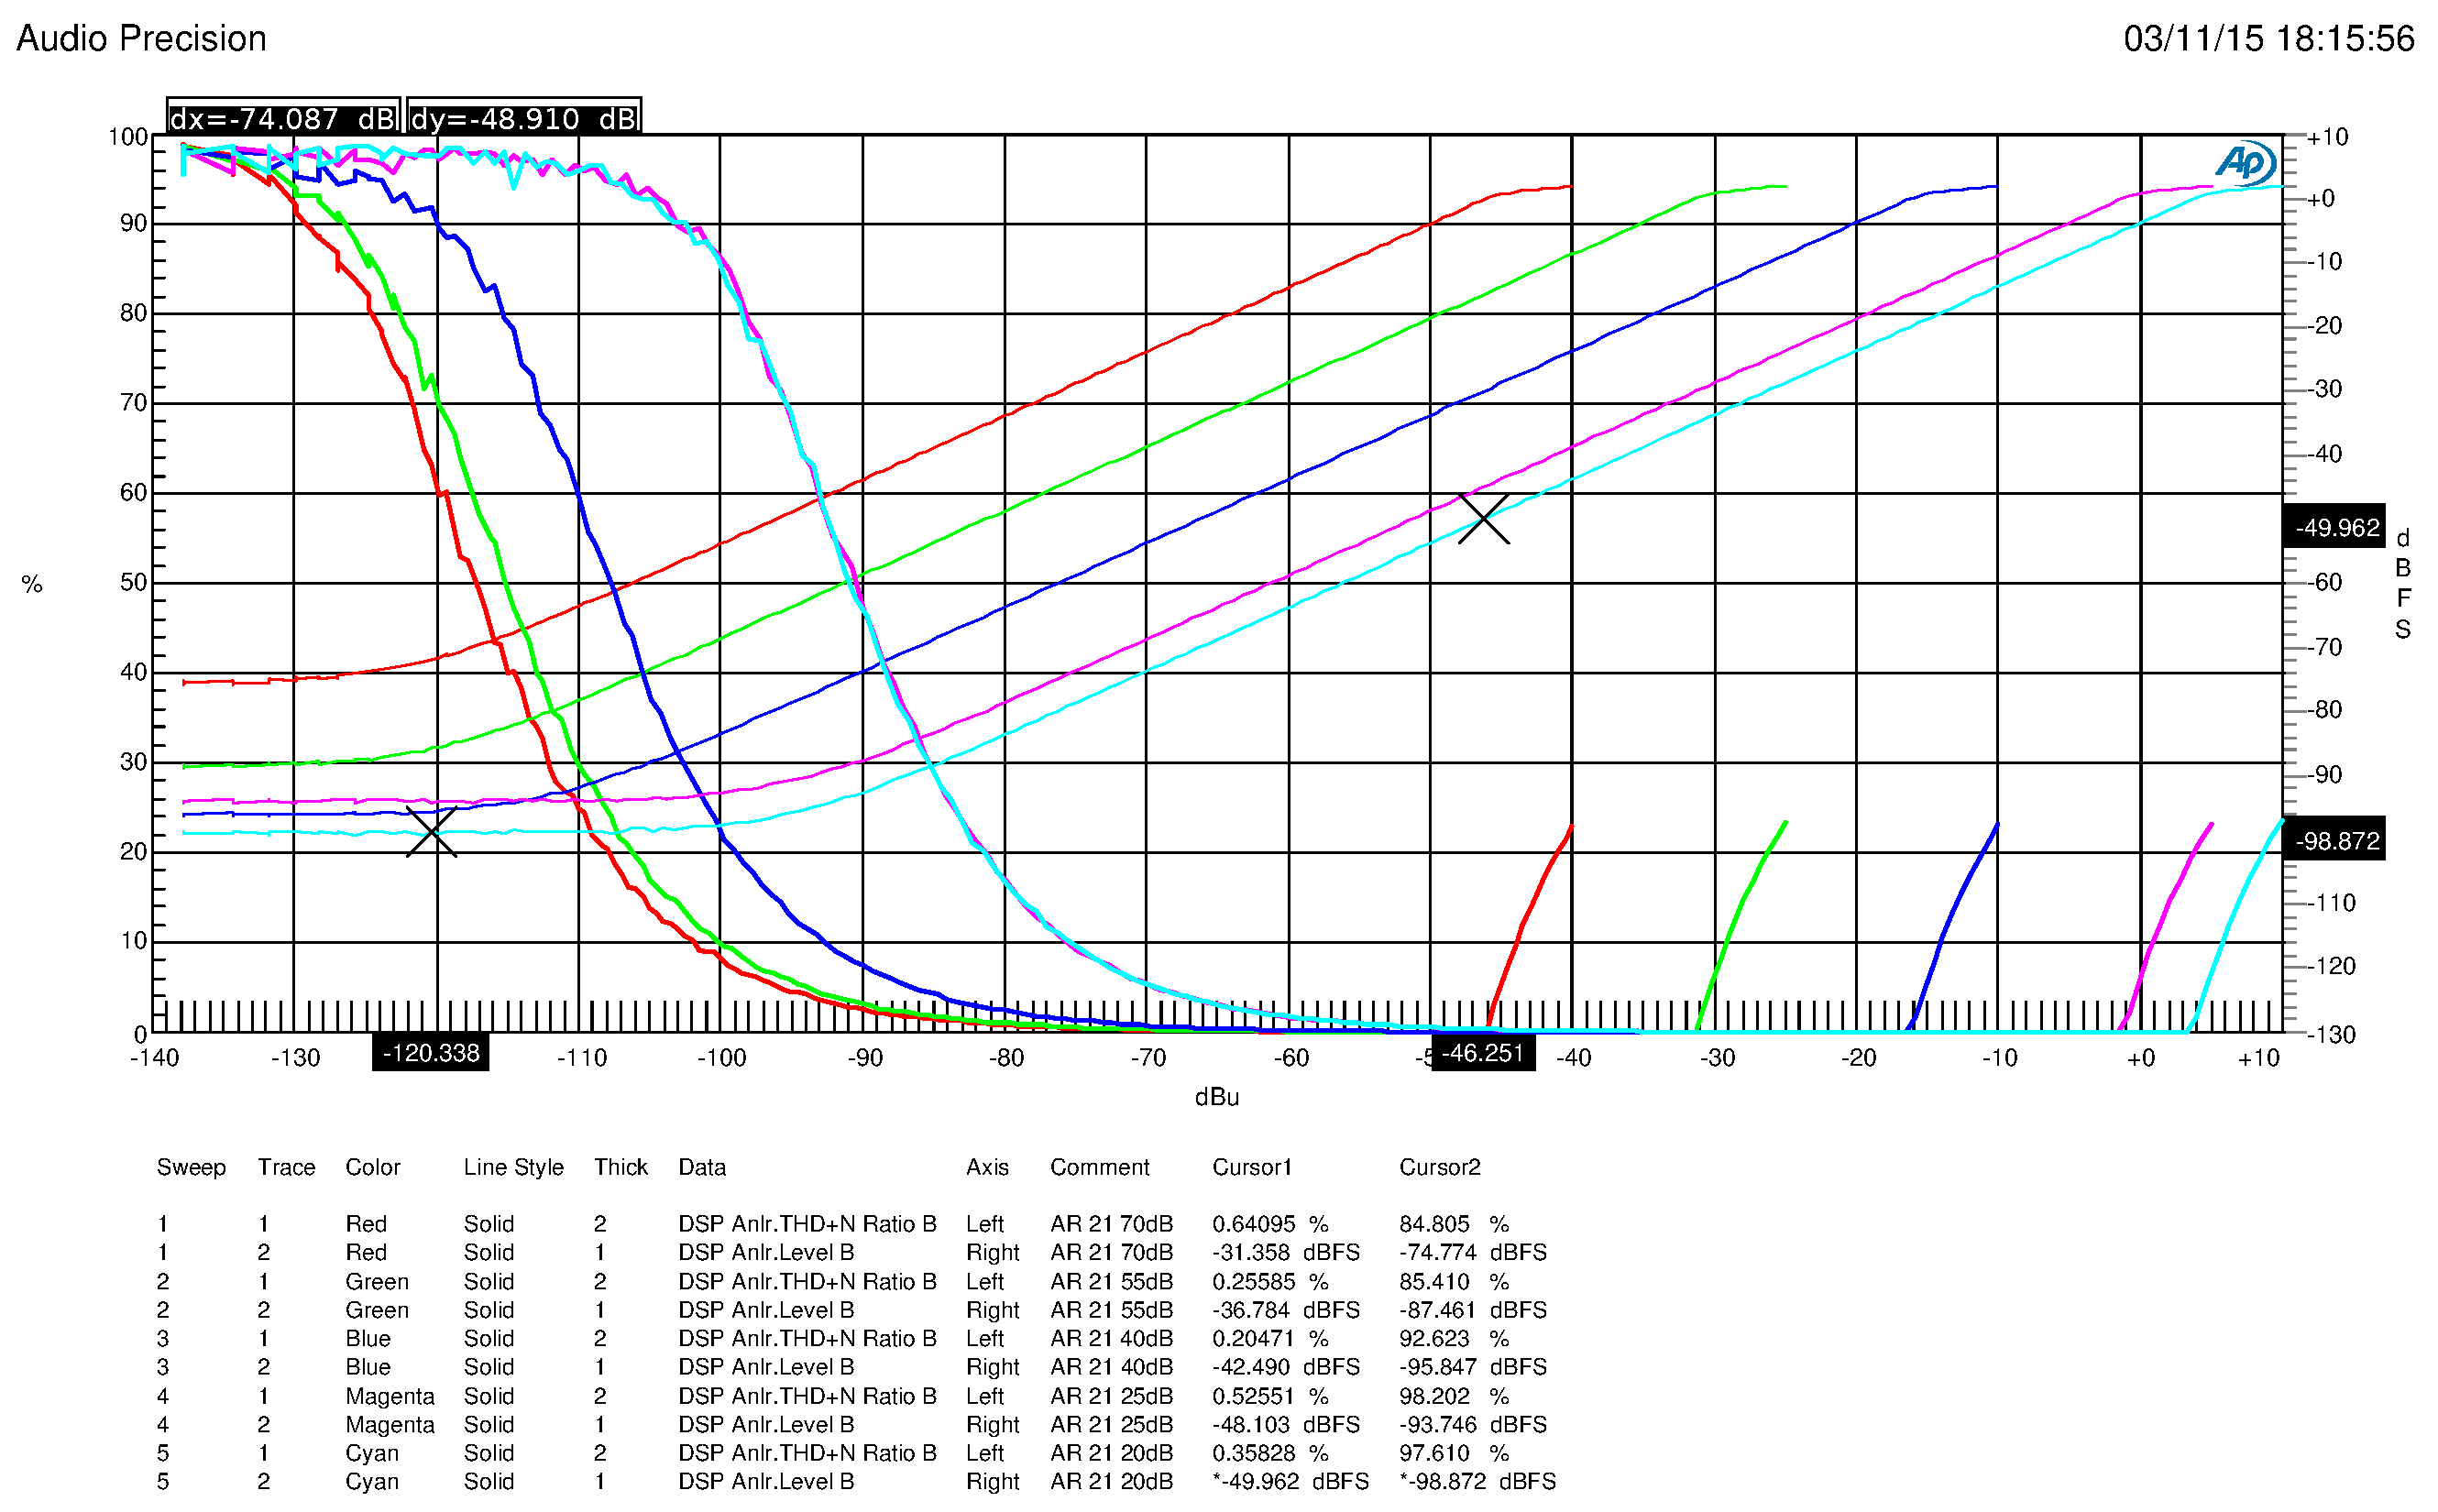
\includegraphics[width=14cm,keepaspectratio=true]{THDAR21dBVergleich}
\caption{dynamic range of channel AR21}
\label{fig:adthd}
\end{center}
\end{figure}

\begin{figure}[htbp]
\begin{center}
\includegraphics[width=14cm,keepaspectratio=true]{THDAR5HQdBVergleich}
\caption{dynamic range of high quality channel AR5}
\label{fig:adhqthd}
\end{center}
\end{figure}

	\subsection{Discussion}
It can be easily obtained in figures \ref{fig:adlawo} and \ref{fig:adlawovergleich} that both ADCs have a very flat frequency response over the whole frequency range. A steep slope down can be seen at half of the sampling frequency. The standard quality input has less amplification of low amplitudes, but at a very low frequency and with inegligible difference.\\
In figure \ref{fig:adthd} the THD+N as well as the dynamic range of the standard definition microphone input at different preamplifier gains are shown.  The input is straight linear at every preamplifier gain. The THD shown on the left side increases with lower amplifier gain, but also the noise floor is lower. The lower the preamplifier gain is the higher the dynamic range. On the right side a steep increasing distortion can be obtained. Dynamic ranges are shown in tabular \ref{ŧab:amplgains}.\\
Figure \ref{fig:adhqthd} show the dynamic range and the THD+N of the high quality microphone input. The noise floor is a little bit lower than with standard quality inputs, but there is almost no audible difference. Dynamic ranges of the high quality microphone input are higher and can be seen for different preamplification gains in tabular \ref{tab:amplgains}.
\begin{table}
\begin{center}
\begin{tabular}{|c||c|c|}
\hline 
preamplification [dB]  & 	dynamic range SQ [dB] & dynamic range HQ [dB]	\\	 \hline
70 &	72 & 81 \\
55 &	84 & 95 \\
40 &	93 & 108	\\
25&	92 & 116 \\
16 (HQ), 20 (SQ) & 97 & 122\\
\hline
\end{tabular}
\caption{dynamic ranges and THD+N for standard and high quality microphone inputs and analog-digital conversion}
\label{tab:amplgains}
\end{center}
\end{table}
\begin{leftbar}
\textit{Note:\\
When converting a digital signal to the analog domain a maximum of $+3dB_{FS}$ is possible, but at this area distortions occur.}
\end{leftbar}

%---------------------------------------------------------------------------------------------------------
%---------------------------------------------------------------------------------------------------------
\chapter{Conclusion}
In this laboratory exercise the measurement of ADCs and DACs with AudioPrecision was done. It showed some smaller differences between SQ and HQ inputs and outputs, but parameters does not change dramatically. In further measurements other inputs and outputs can be measured and filters can be included to measurements. Filter measurements  were done on an other laboratory day. Concluding this exercise helps to understand the main functionality of ADCs and DACs and the important parameters of these converting elements.




\begin{appendix}
\nomenclature{ADC}{analog to digital converter}
\nomenclature{DAC}{digital to analog converter}
\nomenclature{THD}{total harmonic distortion}
\nomenclature{THD+N}{total harmonic distortion including noise}
\nomenclature{HQ}{high quality}
\nomenclature{AP}{AudioPrecision}
\nomenclature{AR}{Aufnahmeraum, audio studio TU Graz}
\nomenclature{RP1}{Regieplatz 1, audio studio TU Graz}
\nomenclature{SSL}{Solid State Logic}
\nomenclature{DALLIS}{Digital Audio Line Level Interface System}
\nomenclature{$dB_{FS}$}{dB Full Scale}
\nomenclature{SQ}{Standard Quality}




\chapter{High resolution diagrams}
\begin{figure}[htbp]
\begin{center}
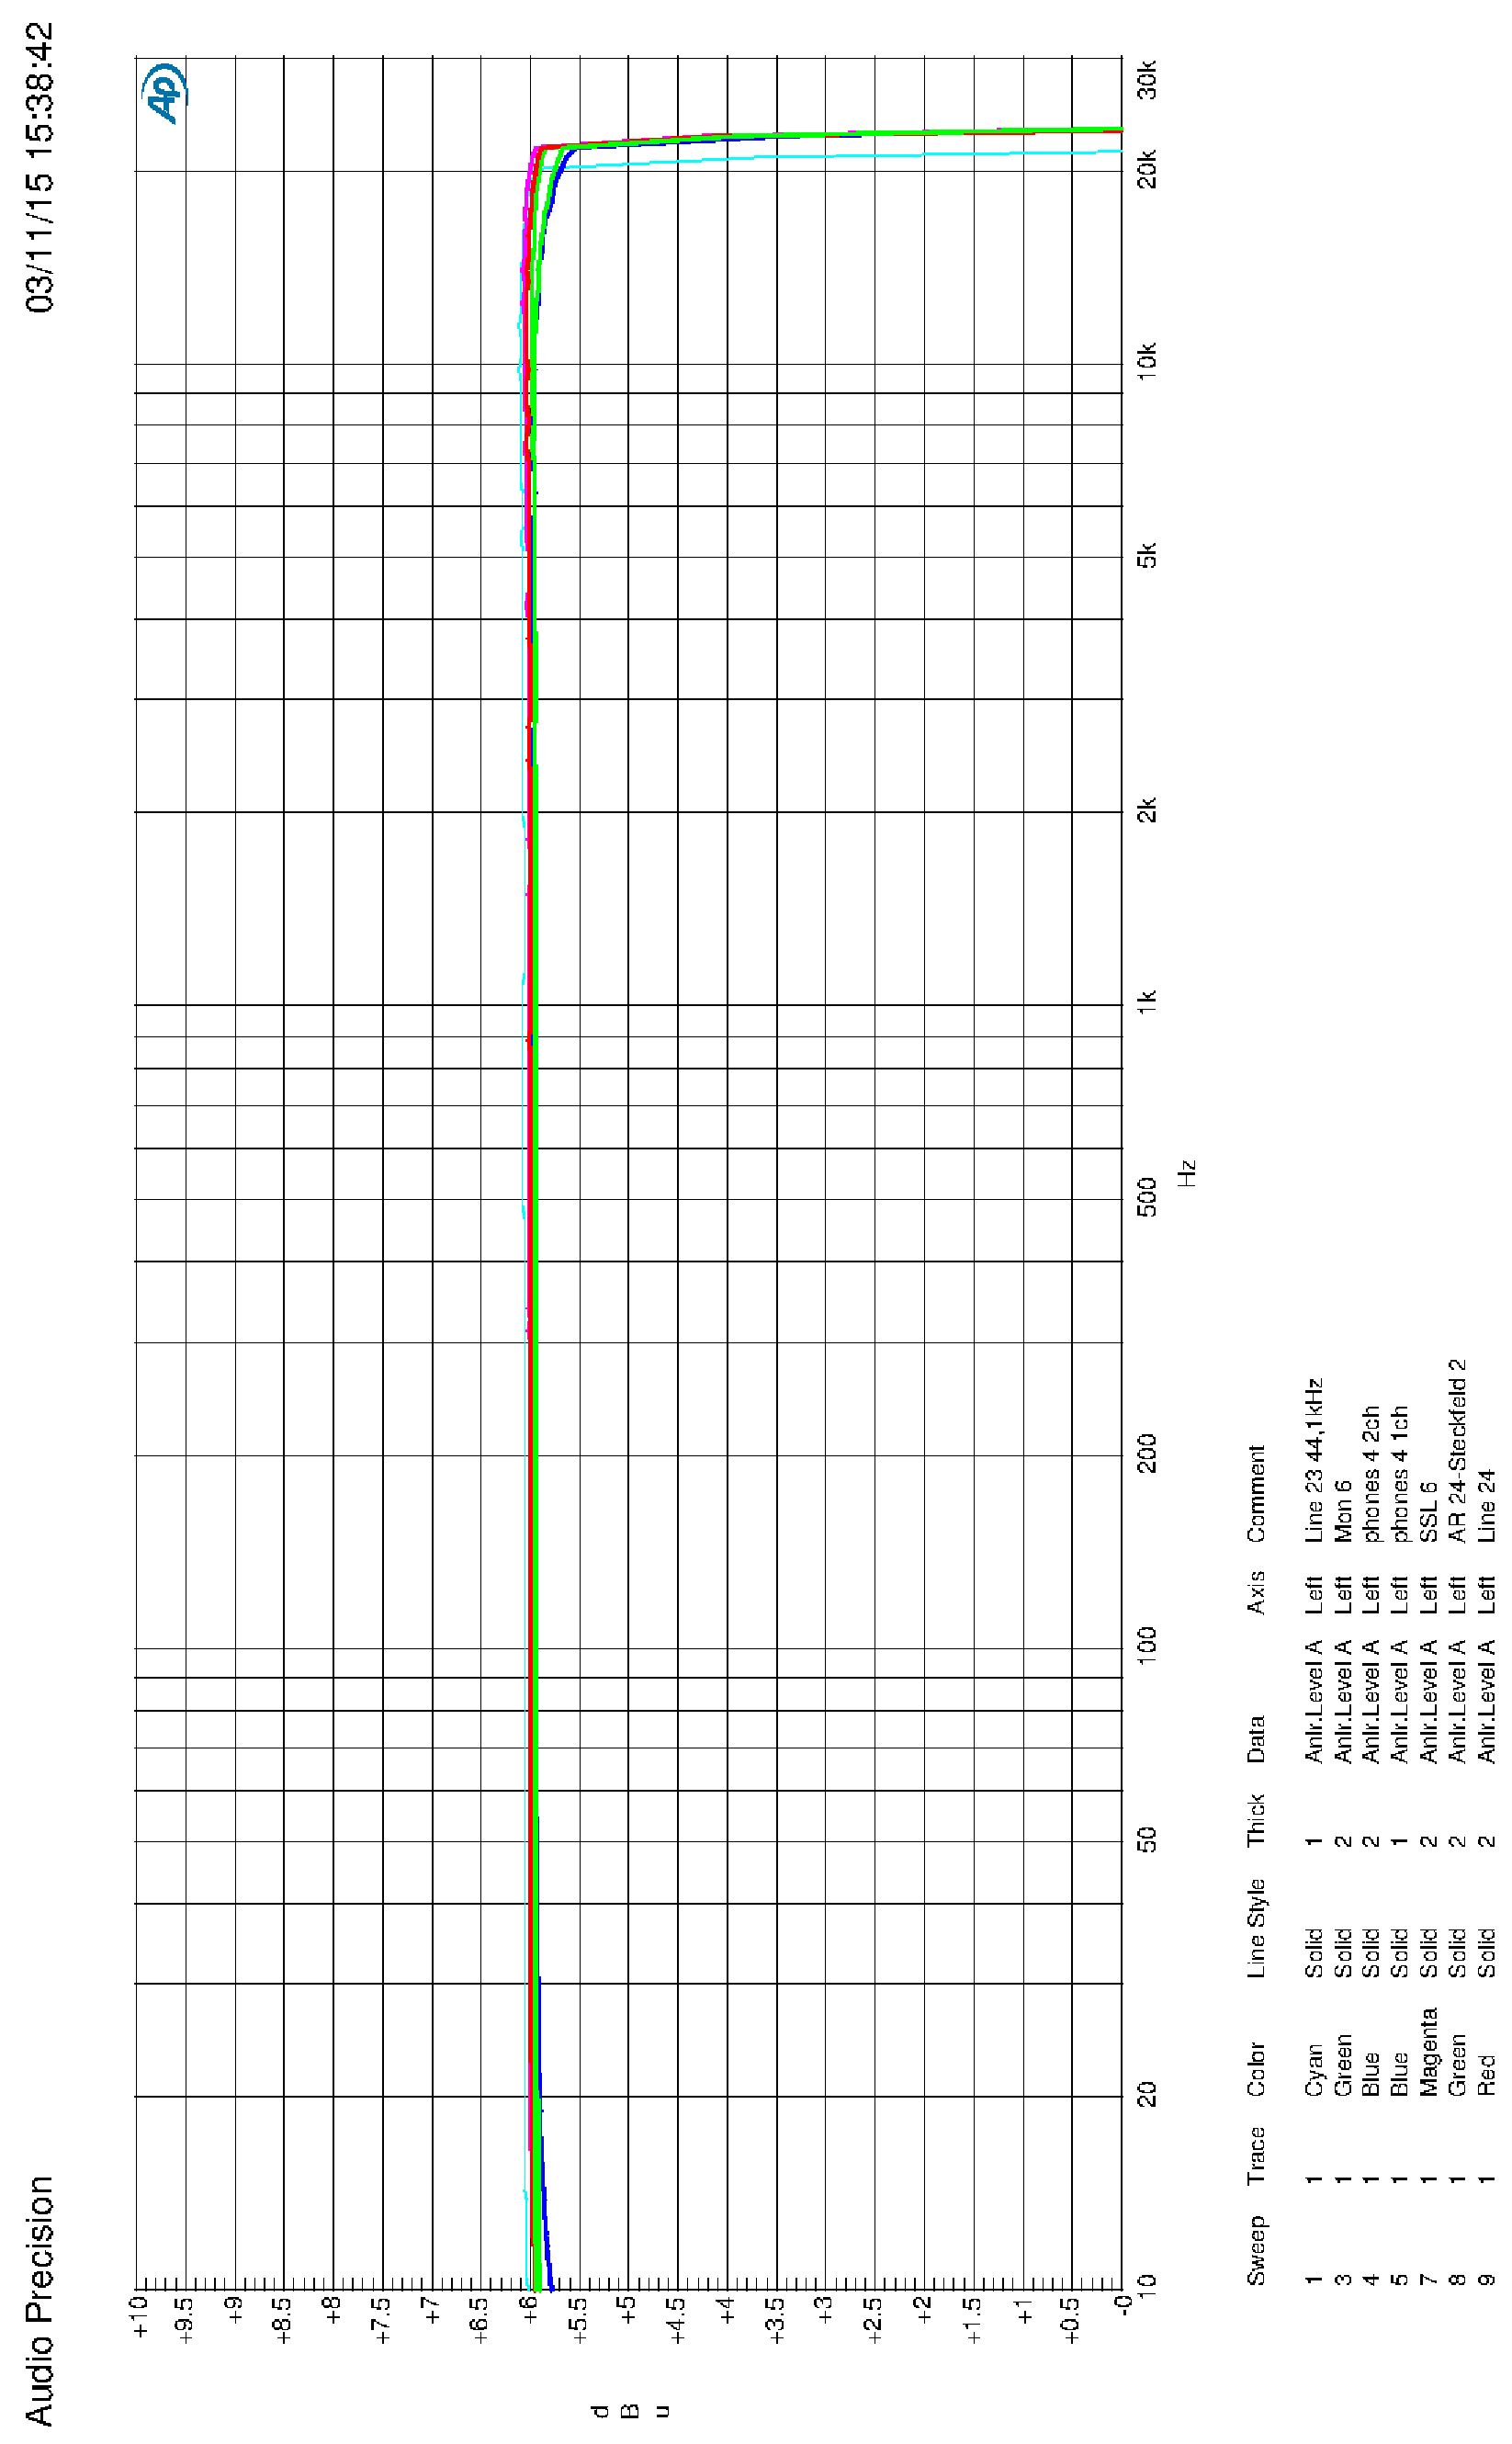
\includegraphics[width=14cm,keepaspectratio=true]{HQDAWandlerVergleich10dB}
\caption{frequency responses of different DACs (high resolution)}
\label{Abb.:1}
\end{center}
\end{figure}



\begin{figure}[htbp]
\begin{center}
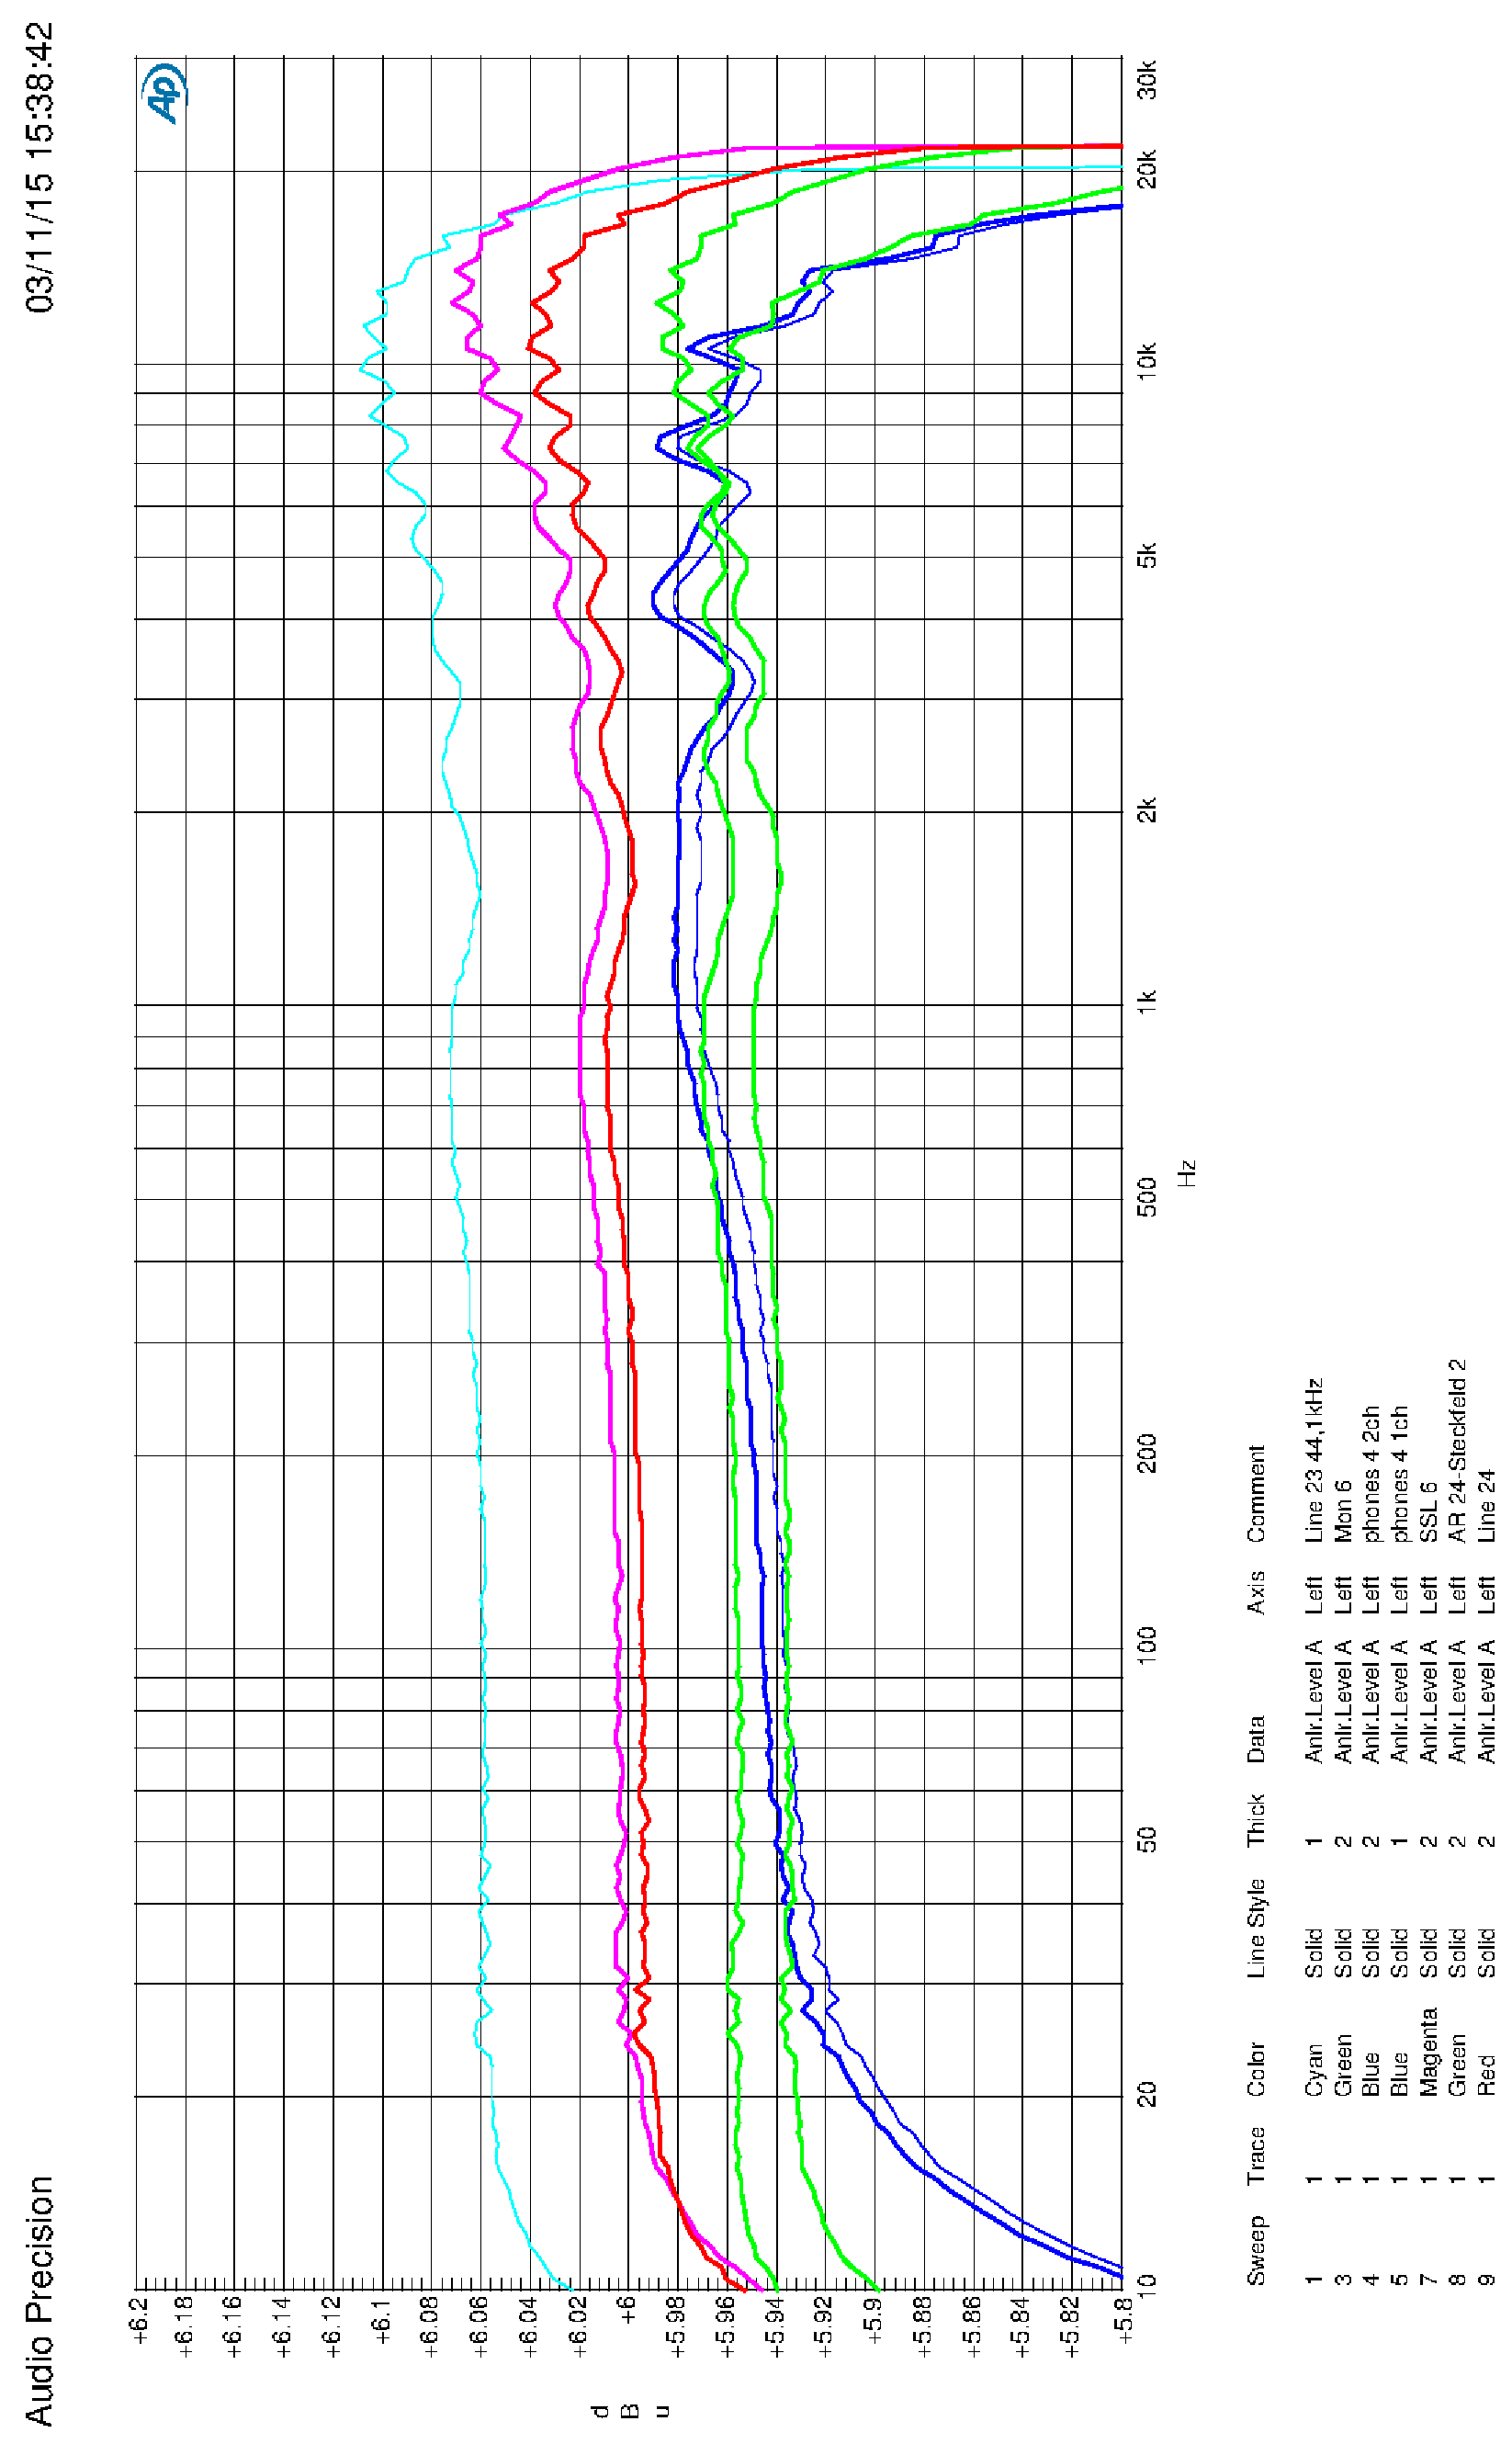
\includegraphics[width=14cm,keepaspectratio=true]{HQDaWandlerVergleich}
\caption{detailed frequency responses of different DACs (high resolution)}
\label{Abb.:1}
\end{center}
\end{figure}

\begin{figure}[htbp]
\begin{center}
\includegraphics[width=14cm,keepaspectratio=true]{HQDynamikvergleich}
\caption{dynamic ranges of different DACs (high resolution)}
\label{Abb.:1}
\end{center}
\end{figure}

\begin{figure}[htbp]
\begin{center}
\includegraphics[width=14cm,keepaspectratio=true]{HQFFTrauschen}
\caption{FFT of line24 signal (high resolution)}
\label{Abb.:1}
\end{center}
\end{figure}

\begin{figure}[htbp]
\begin{center}
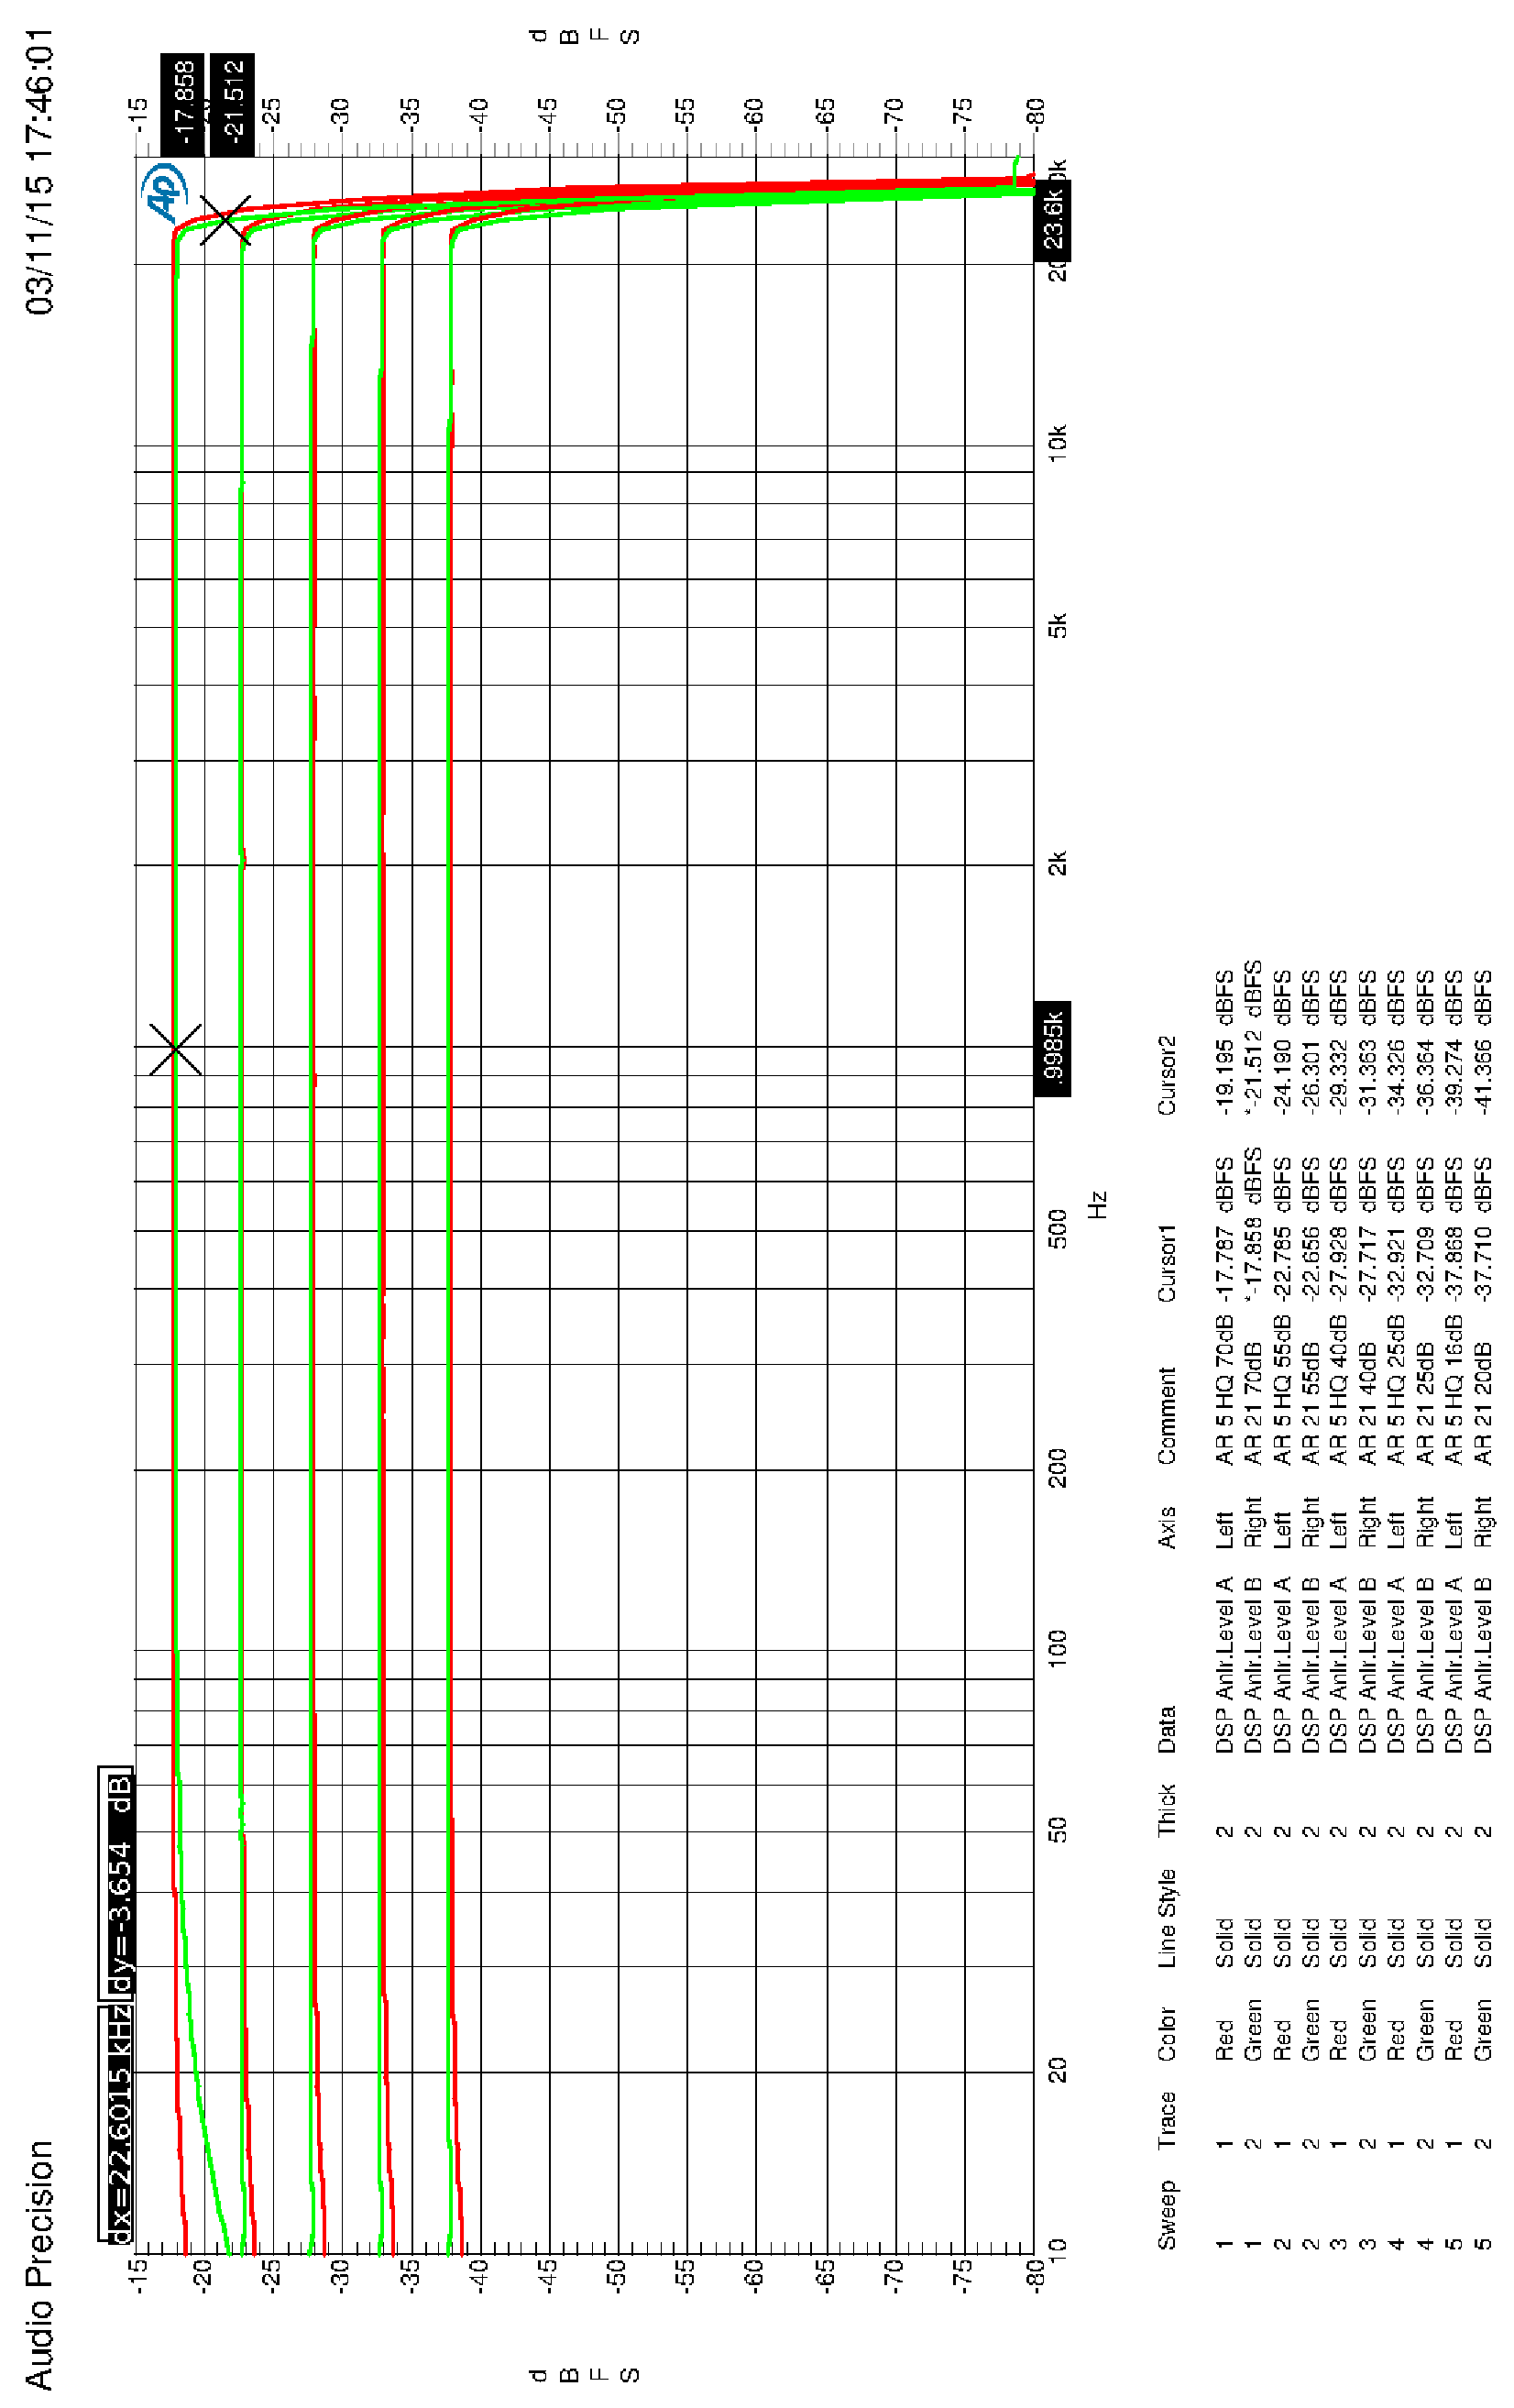
\includegraphics[width=14cm,keepaspectratio=true]{HQLAWOVorverstaerker5u21dB}
\caption{LAWO ADC and preamplifier (high resolution)}
\label{Abb.:1}
\end{center}
\end{figure}

\begin{figure}[htbp]
\begin{center}
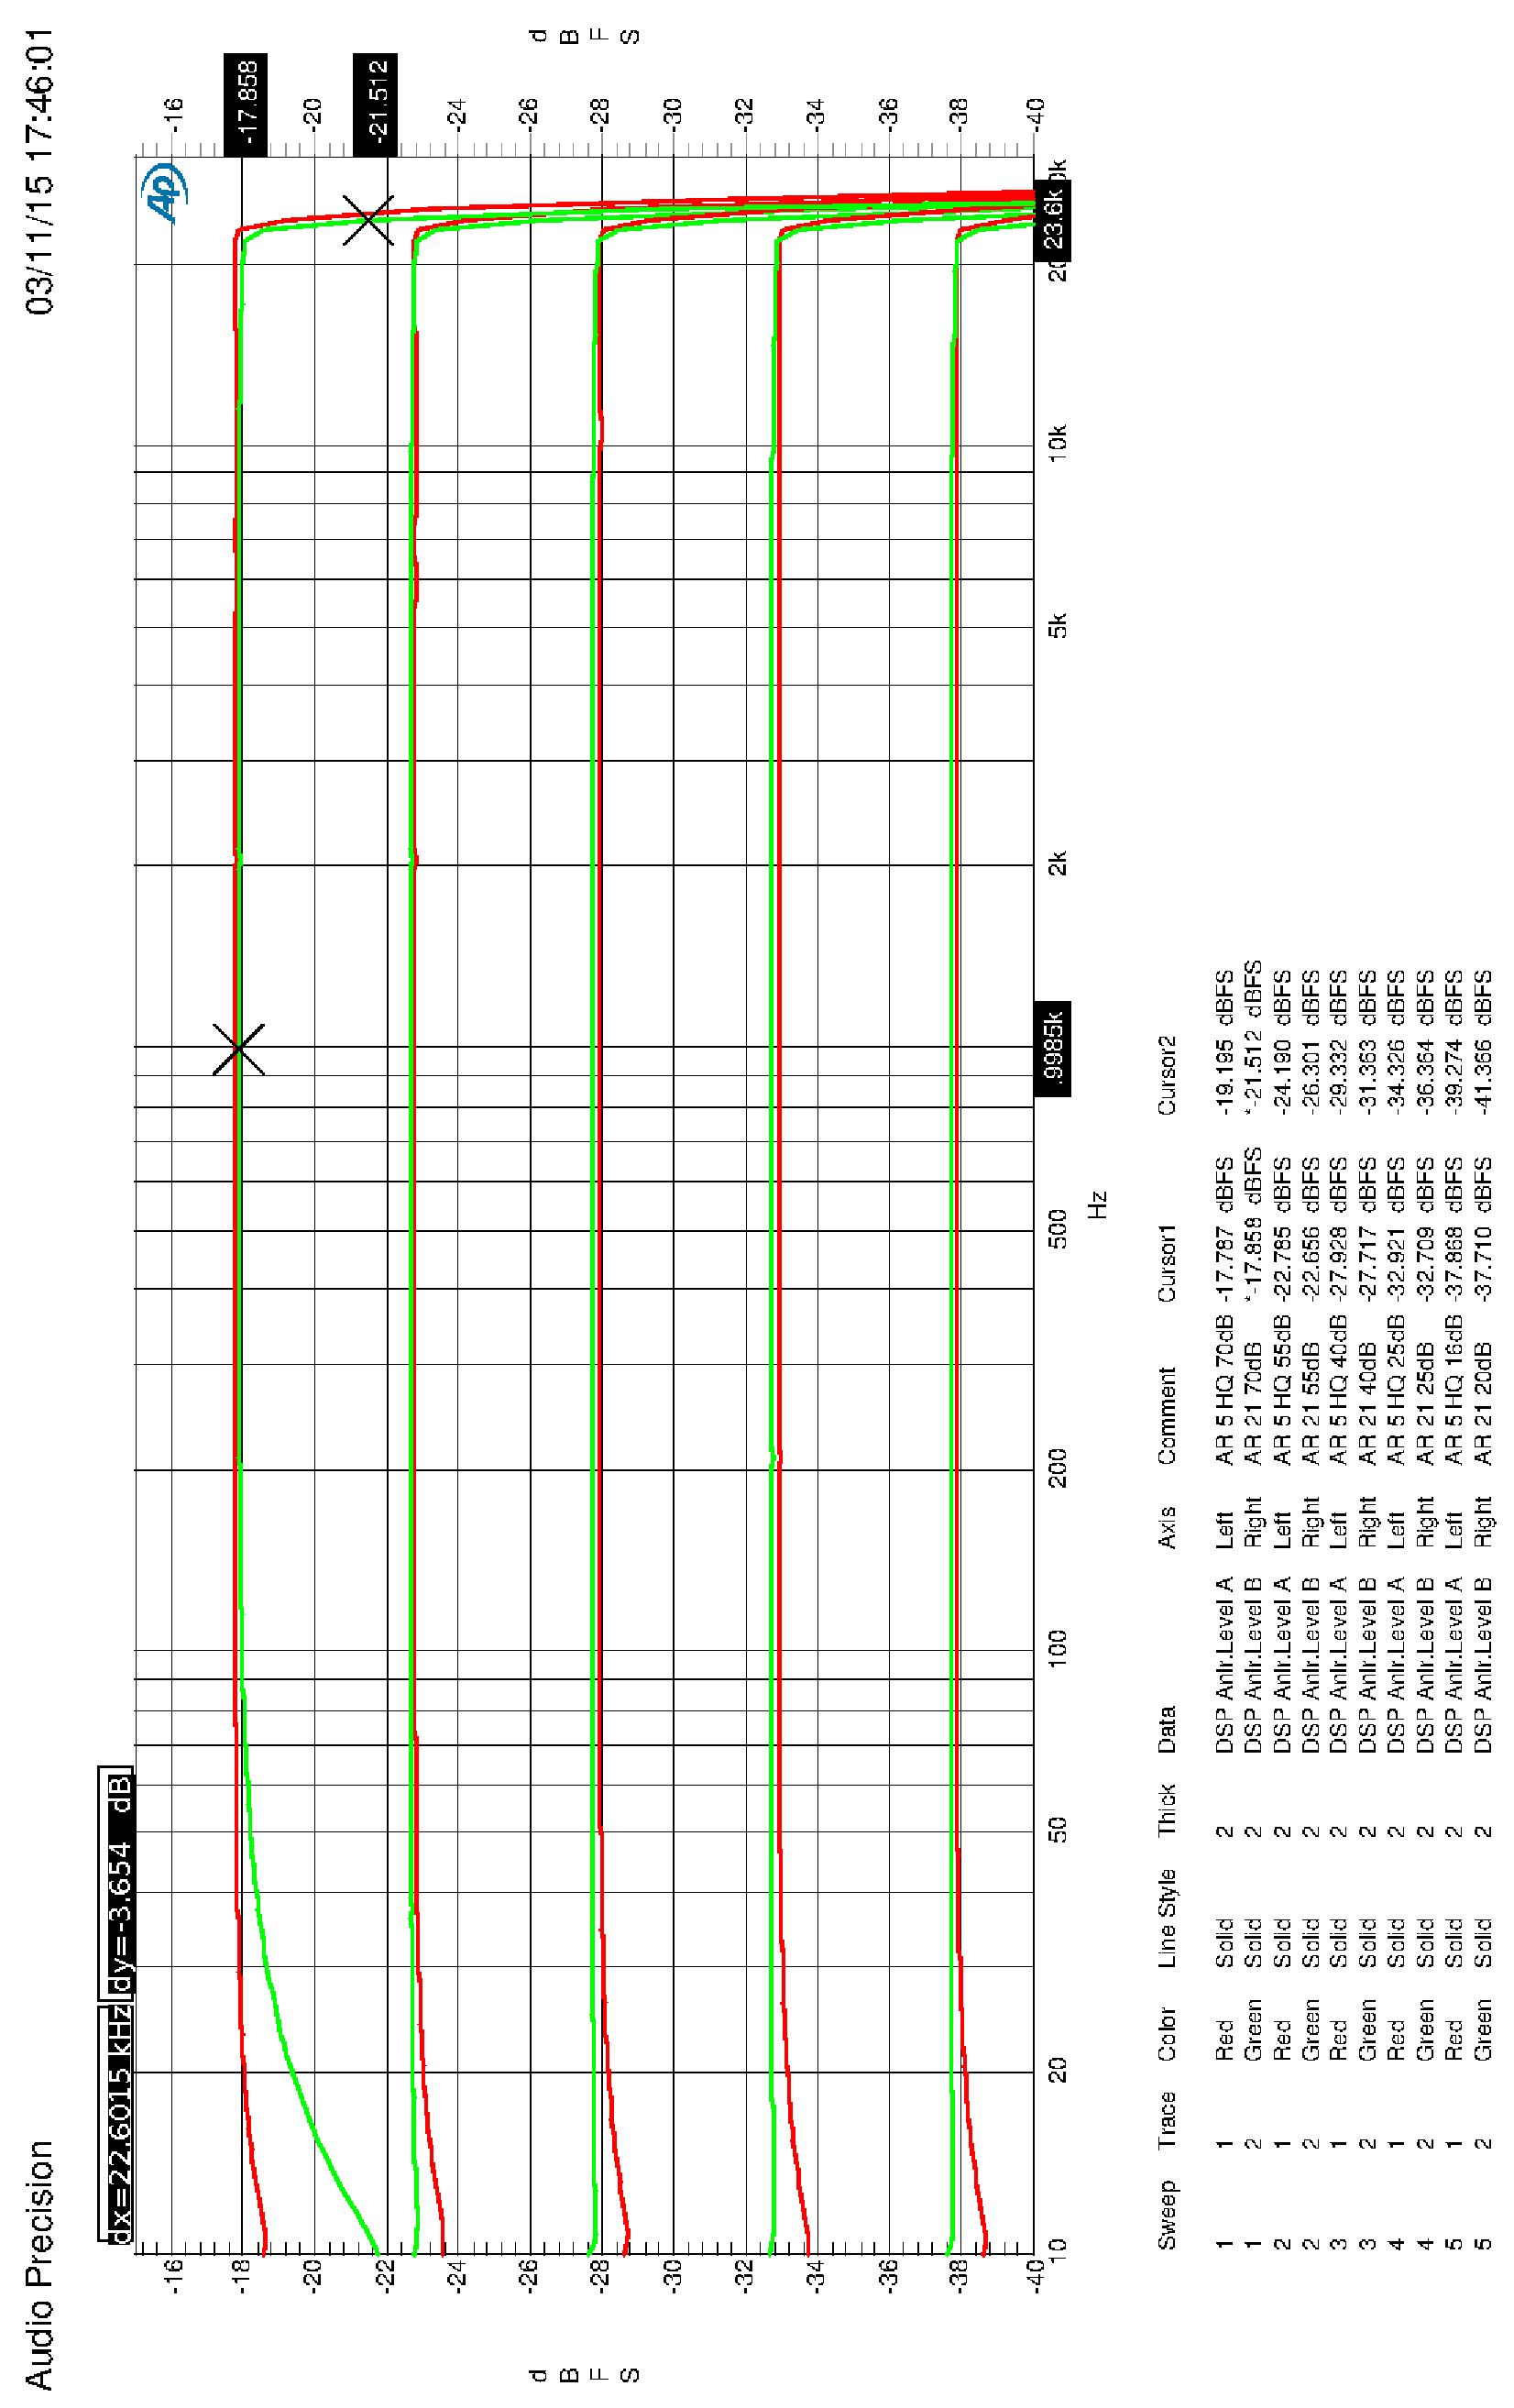
\includegraphics[width=14cm,keepaspectratio=true]{HQLAWOVorverstaerker5u21dBVergleichszoom}
\caption{LAWO ADC and preamplifier detailed view (high resolution)}
\label{Abb.:1}
\end{center}
\end{figure}

\begin{figure}[htbp]
\begin{center}
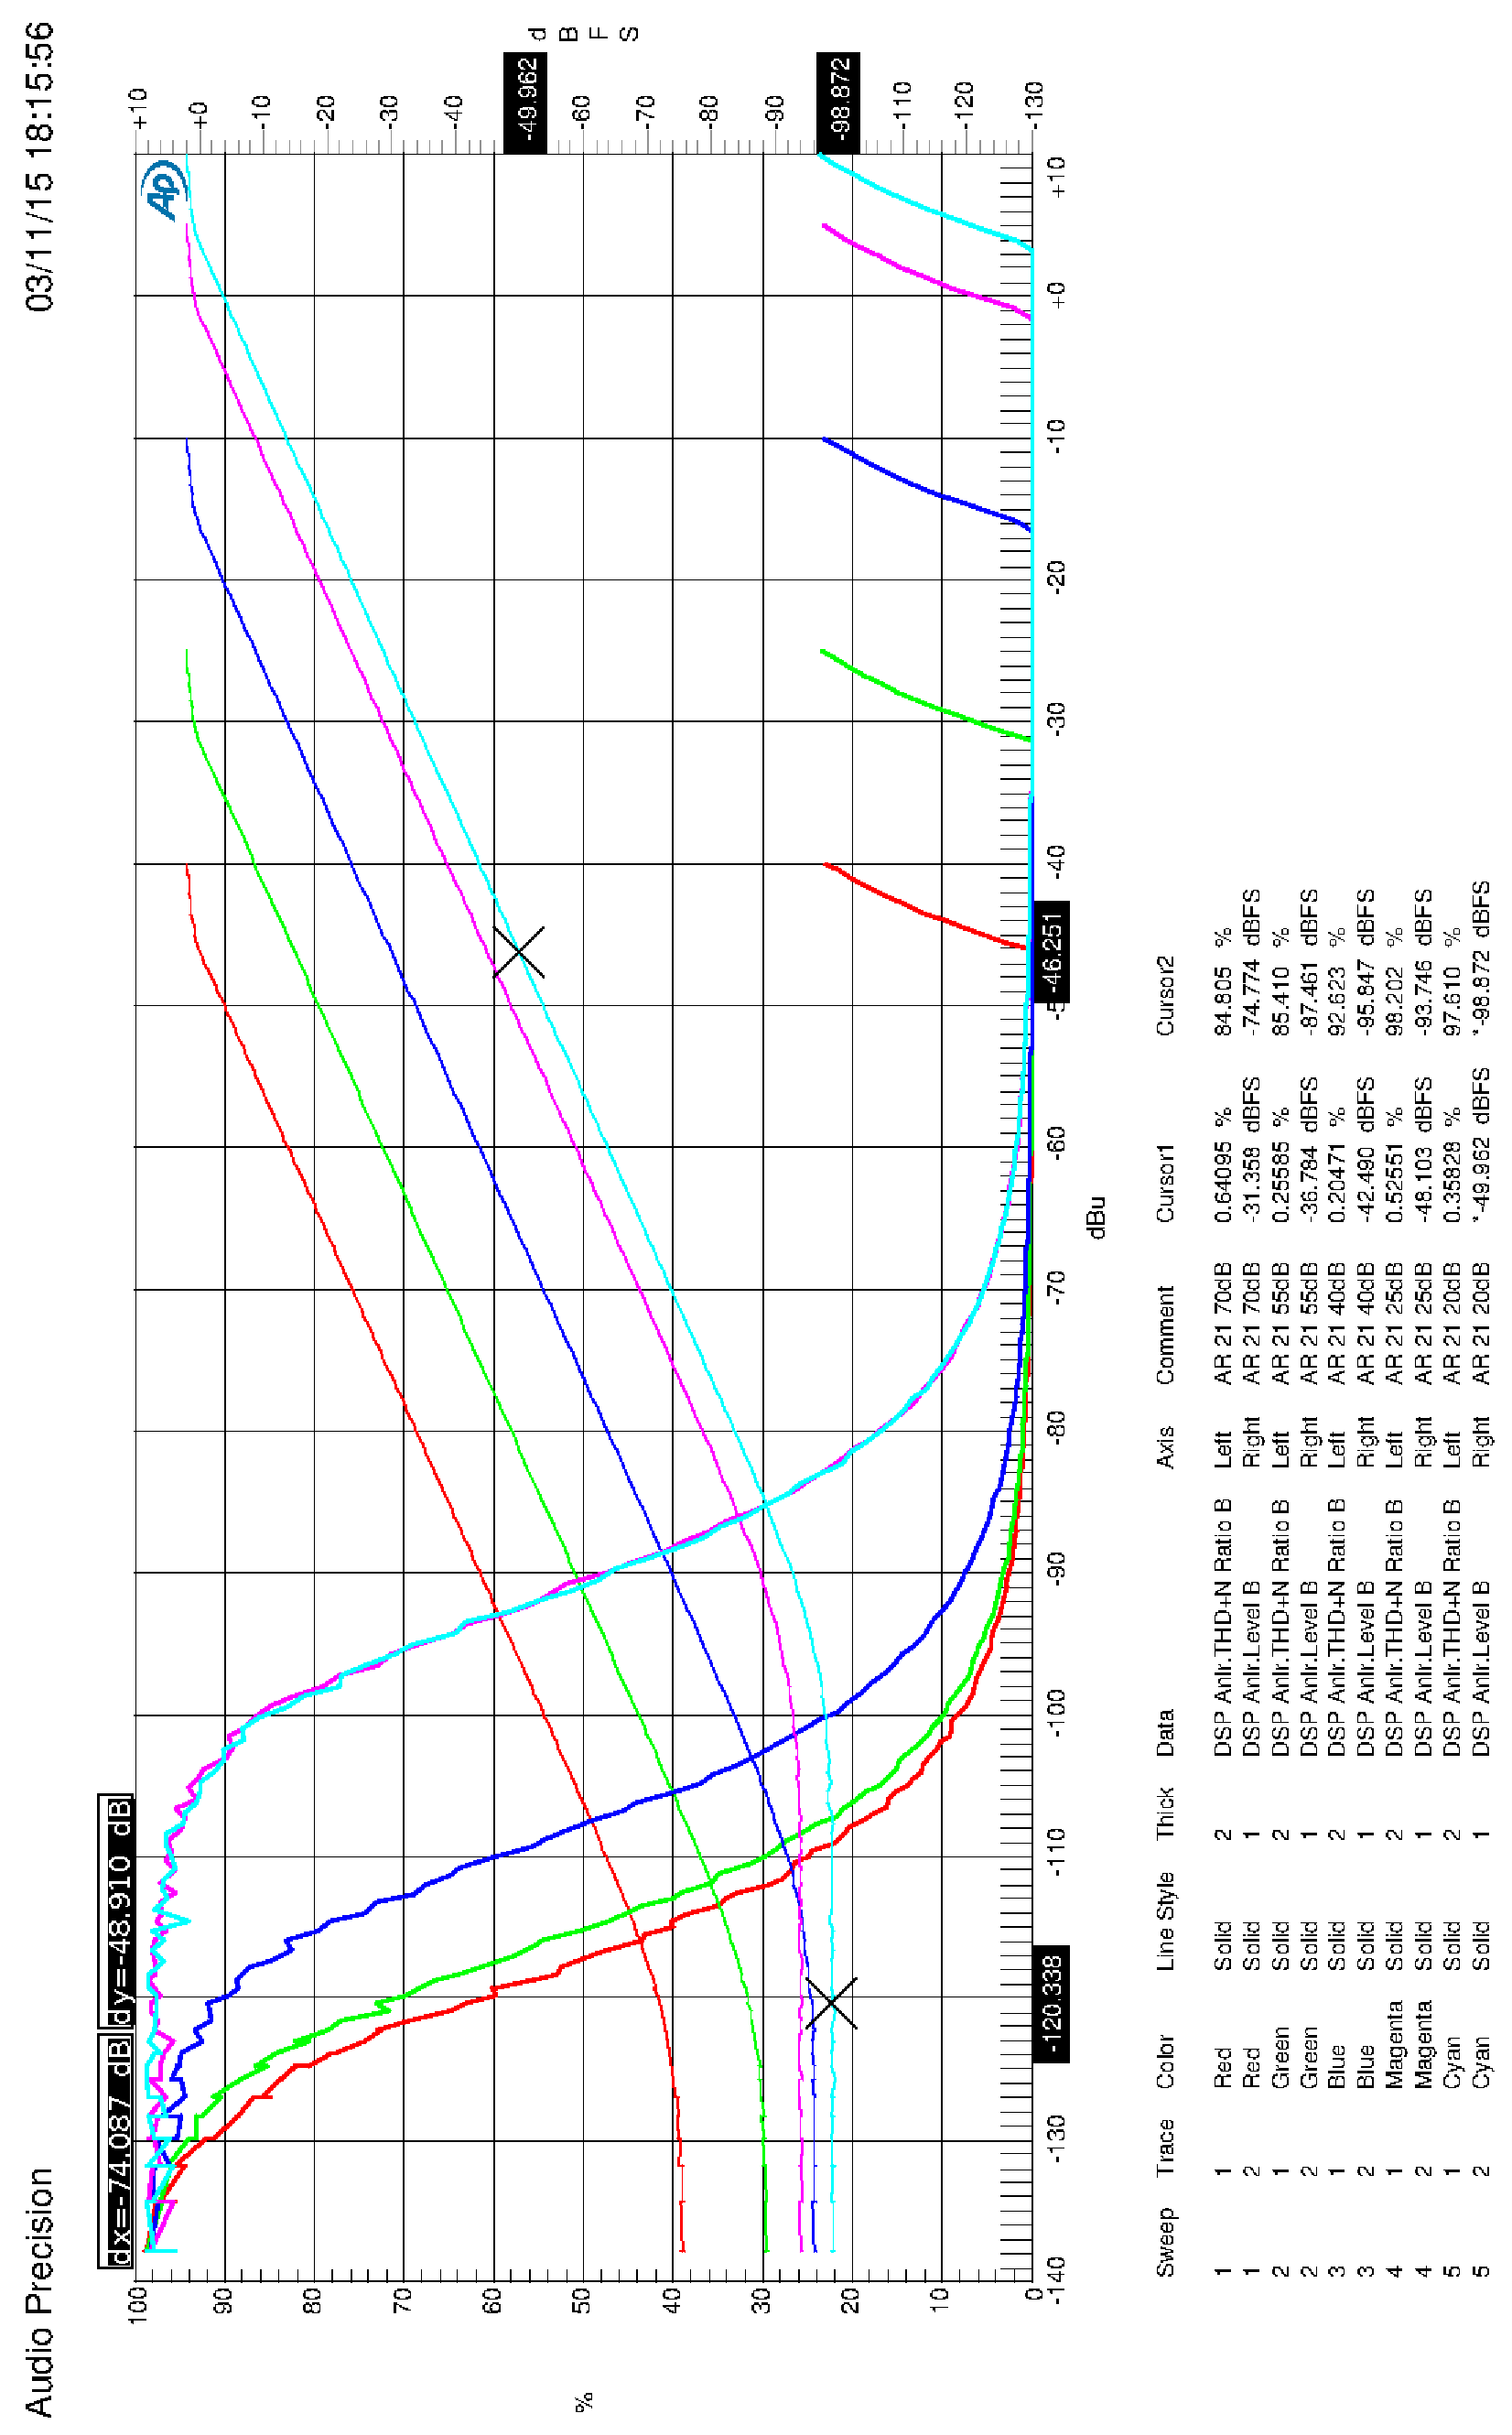
\includegraphics[width=14cm,keepaspectratio=true]{HQTHDAR21dBVergleich}
\caption{dynamic range of channel AR21 (high resolution)}
\label{Abb.:1}
\end{center}
\end{figure}

\begin{figure}[htbp]
\begin{center}
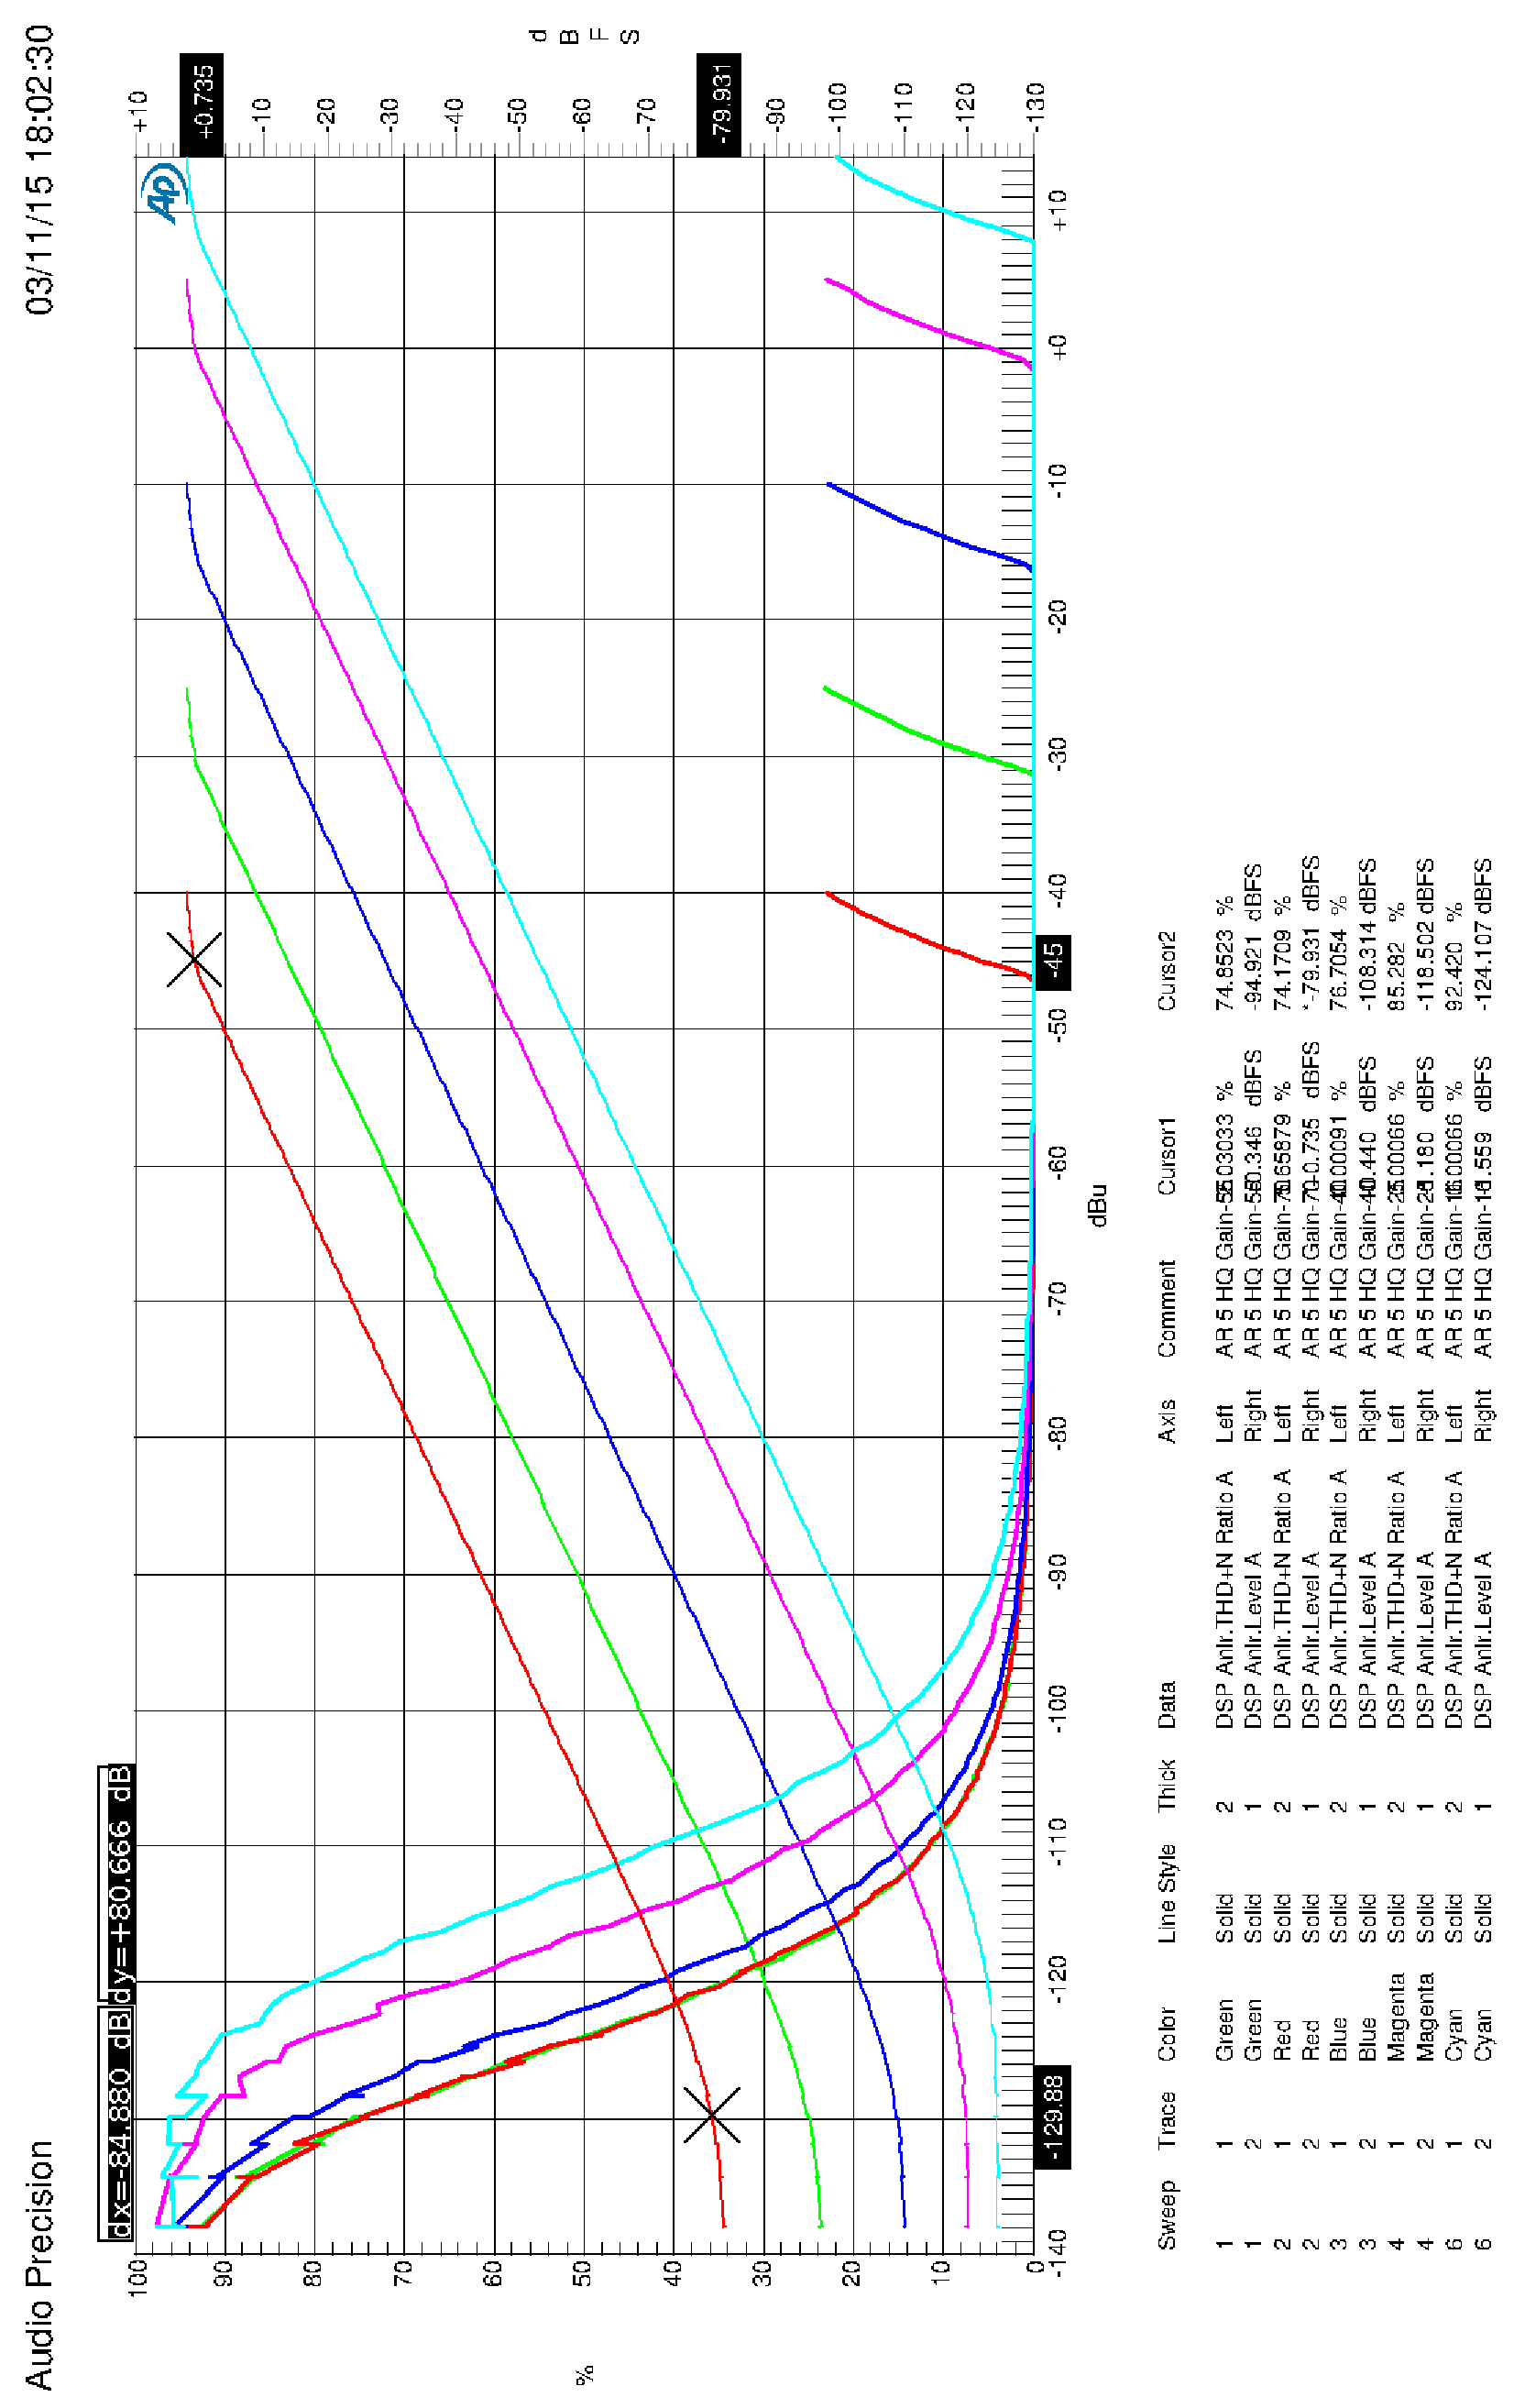
\includegraphics[width=14cm,keepaspectratio=true]{HQTHDAR5HQdBVergleich}
\caption{dynamic range of high quality channel AR5 (high resolution)}
\label{Abb.:1}
\end{center}
\end{figure}









\printnomenclature

\end{appendix}

%nicht referenzierte Literaturstellen

\nocite{mseifter88,pmandl97,weiss92,weiss92a,ginthoer93}

% Literaturverzeichnis einbinden, alpha, plain, unsrt, abbrv
\newpage
%Eintrag im Inhaltsverzeichnis
\addtocounter{page}{1}
\addcontentsline{toc}{chapter}{Literaturverzeichnis}
\addtocounter{page}{-1}

\bibliographystyle{alpha}

\bibliography{protokoll}

%Index File
%\input{diplom.ind}

\end{document}
